%some-literature review


In the last few decades, several scientists have modeled the dynamics and ecological impact of marine aggregates \cite{jackson_aggregation_1998, kiorboe_mechanisms_2002}. 
Their effects on bacterial transport \cite{jackson_simulation_1989} and algal bloom \cite{jackson_model_1990} have been described in models that use simplified descriptions of the aggregates' settling speeds. Moreover, accumulation of aggregates in thin layers where the ambient fluid is stratified have been reported \cite{macintyre_accumulation_1995, alldredge_occurrence_2002} and more recently modeled experimentally \cite{prairie_delayed_2013}, analytically \cite{camassa_retention_2013}, and computationally \cite{panah_simulations_2017}. Understanding the formation and persistence of these thin layers is ecologically important. 
Therefore, in this chapter, we discuss the dynamics of settling marine aggregates in a density stratified fluid. 
%---------------------------------------------------------
\par
Instead of constant density $\rho$, we suppose the background fluid density varies linearly in the vertical direction,
\begin{equation}
\rho_{bg}(z) =  \rho_0 \left(1 + \gamma z \right),
\label{eq_rho_bg}
\end{equation}
where $\rho_0$ is the fluid density where the aggregate's center of mass is located at rest, and $\gamma$ is constant.
Over the time $t$, some perturbations, $C(\vec{y},t)$, occur due to the concentration, $\tilde{S}(\vec{y},t)$, difference between the background fluid and settling aggregate,
\begin{equation}
C(\vec{y}, t) =  \tilde{S}(\vec{y},t) - \rho_{bg}(z).
\label{eq_perturb_C}
\end{equation}
From equations (\ref{eq_rho_bg}) and (\ref{eq_perturb_C}), we can establish the fluid density variation over time,
\begin{equation}
	\rho(\vec{y},t ) 
	= \rho_{bg}(z) +  \alpha \rho_0 C(\vec{y},t) 
	 = \rho_0 \left( 1 + \gamma z  + \alpha  C(\vec{y},t) \right),
\label{eq_density}
\end{equation}
where the non-zero constant $\alpha $ describes type of solute. Knowing that the concentration is the amount of mole per volume, the density of the fluid would differ by the type of solute or chemicals with the same amount of molecules.
\begin{figure}[ht]
	\begin{center}
	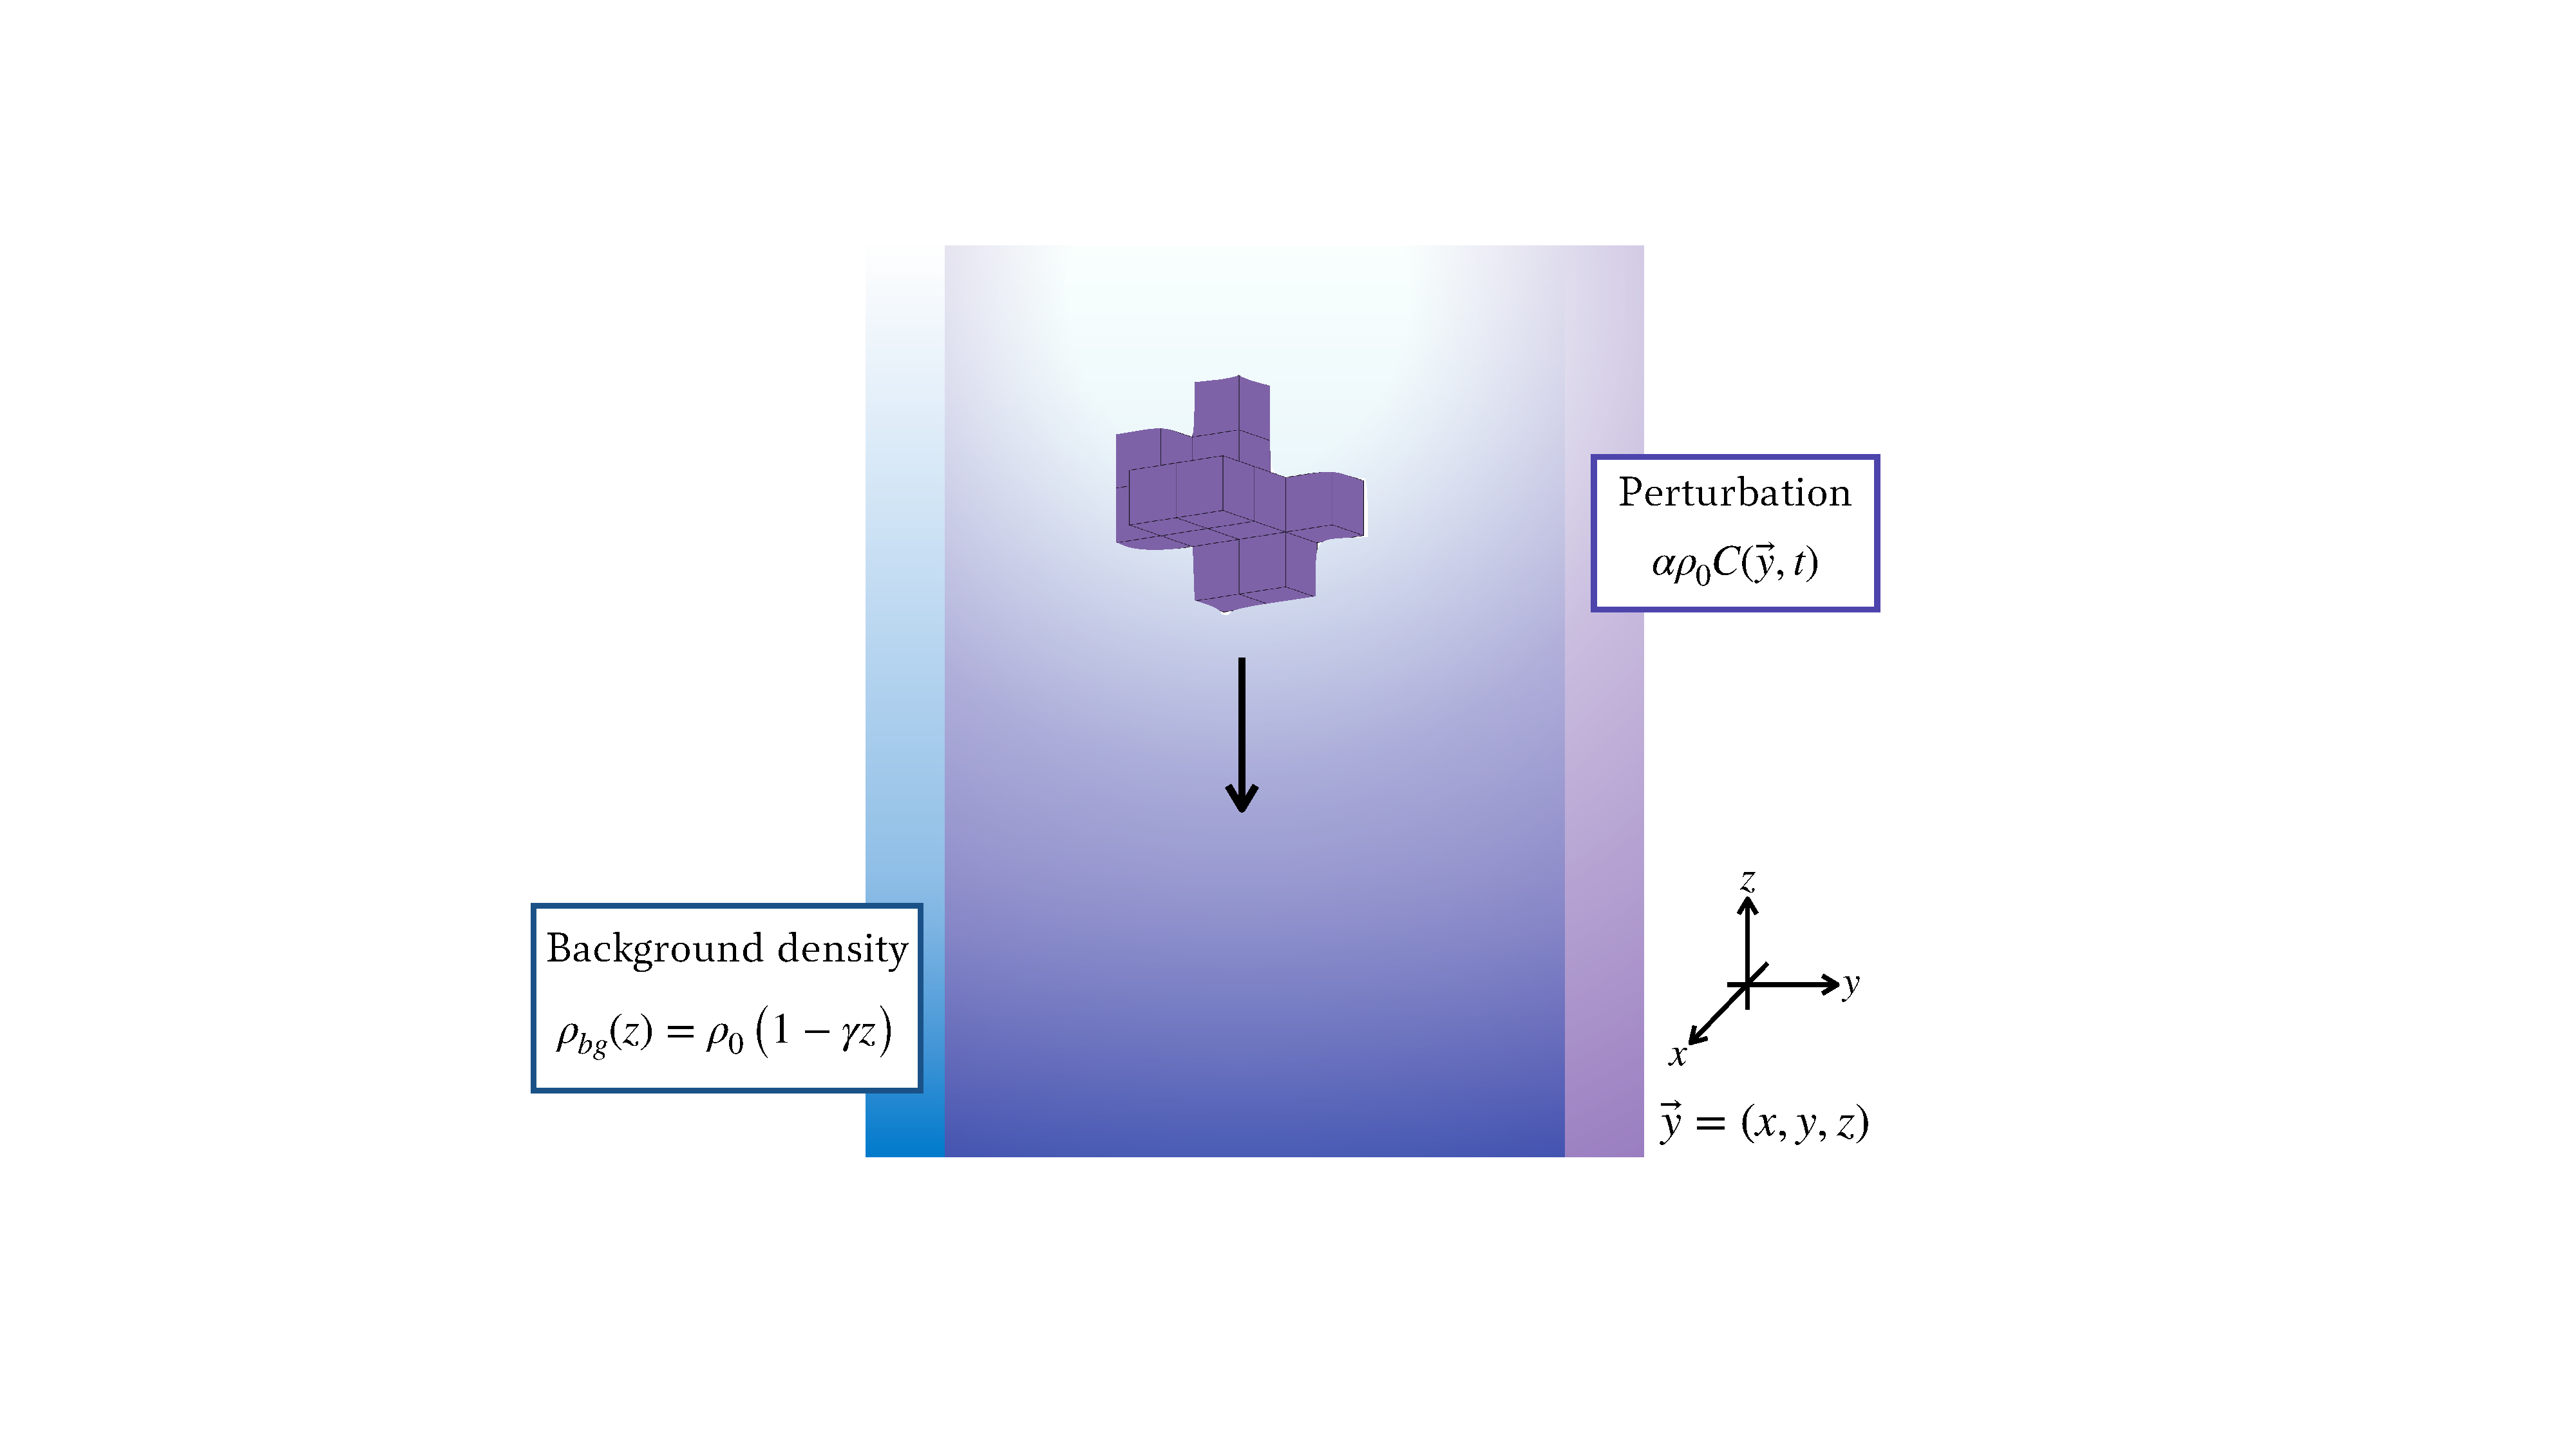
\includegraphics[scale=0.4]{./figures/fig_stratification_schematics}
	\caption{Description of fluid density stratification.}
	\label{fig_stratification_schematics}
	\end{center}
\end{figure}
To track the perturbation $C(\vec{y},t)$, we couple the advection-diffusion equation with the modified Stokes equations that we will describe in the next section. 
%------------------------------------------------------------------------------
\section{Governing Equations}
The non-constant density $\rho(\vec{y},t)$ plays a role as an external source of the fluid. This changes the momentum equation,
	Due to varying density, $\rho(\vec{y}, t)$, 
		 \begin{equation}
		\ \tilde{\mu}\nabla^2 \vec{u}(\vec{y})
		- \nabla P_d (\vec{y}) \ + \  
		 \rho_0 \alpha C(\vec{y},t) \vec{g} =0 , 
	\label{eq_extra_C}
	\end{equation}
	where $P_d$ is dynamic pressure, defined as
\begin{equation}
	P_d (\vec{y})
	 = P (\vec{y}) \ - \int \rho_{bg}(z) g   \textrm{d}z.
	\label{eq_Pd}
\end{equation}
To take the perturbation effect into account, we find the particular solution to the momentum equation (\ref{eq_extra_C}). Once we have one, simple addition to the homogenous solution would give us the entire solution due to the linearity of the system. 
\par
% \subsection{Particular solution to Stokes equations with the stratification}
%----------------------------------------------------------------------
To derive the particular solution, we consider the singularly forced Stokes problem \cite{pozrikidis_boundary_1992},
\begin{equation}
	\ \tilde{\mu} \nabla^2 \vec{u}(\vec{y})
	- \nabla P (\vec{y})
	+\vec{q} \ \delta \left(\vec{x} - \vec{y} \right) =0,
\label{eq_single_stokes}
\end{equation}
where $\vec{q}$ is an arbitrary constant vector, $\vec{y}$ is an arbitrary point in fluid domain, and $\delta$ is the three-dimensional delta function.
The problem (\ref{eq_single_stokes}) 
describes the effect coming from a single force applied at $\vec{x} = \vec{y}.$
The fundamental solutions to equation (\ref{eq_single_stokes}) with the continuity equation are
\begin{equation}
	\vec{u} (\vec{y}) = \ \frac{1}{8\pi \tilde{\mu}}  \bar{\bar{G \ }}(\vec{x}, \vec{y})
	\cdot  \vec{q}.
\label{eq_fund_u}
\end{equation}
\begin{equation}
	P (\vec{y}) = \ \frac{1}{4\pi }  
	\frac{\vec{x} - \vec{y}}{\| \vec{x} - \vec{y}\|^3}
	\cdot  \vec{q},
\label{eq_fund_p}
\end{equation}
where the kernel $\bar{\bar{G \ }}$ is called \textit{Stokeslet}, defined as 
\begin{equation}
	\bar{\bar{G}}( \vec{x}, \vec{y}) = 
	\frac{\bar{\bar{I \ }}}{||\vec{x}-\vec{y} ||} + \frac{(\vec{x}-\vec{y})(\vec{x}-\vec{y})^T}{||\vec{x}-\vec{y} ||^3}.
	% \label{eq_stokeslet_repeat}
\end{equation} 
This implies that the solutions (\ref{eq_fund_u}) and (\ref{eq_fund_p}) satisfy equation (\ref{eq_single_stokes}) as
\begin{equation}
	\ \tilde{\mu} \nabla^2 
	\biggl( \frac{1}{8\pi \tilde{\mu}}  \bar{\bar{G \ }}(\vec{x}, \vec{y})
	\cdot  \vec{q} \biggr)
	- \nabla \biggl(\ \frac{1}{4\pi }  
	\frac{\vec{x} - \vec{y}}{\| \vec{x} - \vec{y}\|^3}
	\cdot  \vec{q} \biggr)
	+ \vec{q} \ \delta \left(\vec{x} - \vec{y} \right)
	=0 .
\label{eq_single_stokes_sub}
\end{equation}
As we multiply by $\left( C(\vec{x}, t) \right)$ on both sides and integrate the entire equation over the domain, $V(\vec{x})$, we get
\begin{equation}
	\int_{V}
	\biggl[
	\ \tilde{\mu} \nabla^2 
	\biggl( \frac{1}{8\pi \tilde{\mu}}  \bar{\bar{G \ }}(\vec{x}, \vec{y})
	\cdot  \vec{q} \biggr)
	C(\vec{x}, t)
	-
	\nabla \biggl(\ \frac{1}{4\pi }  
	\frac{\vec{x} - \vec{y}}{\| \vec{x} - \vec{y}\|^3}
	\cdot  \vec{q} \biggr)
	C(\vec{x}, t)
	+ \vec{q} \ \delta \left(\vec{x} - \vec{y} \right)
	C(\vec{x}, t)
	\biggr]
	\ \textrm{d}V(\vec{x}) = 0 .
\label{eq_single_stokes_sub2}
\end{equation}

Note that the operator $\nabla$ is linear and used with respect to $\vec{x}$. We are able to switch the order with the integral operator as follows,
\begin{equation}
	\tilde{\mu} \ \nabla^2 
	\int_{V}
	\biggl( \frac{1}{8\pi \tilde{\mu}}  \bar{\bar{G \ }}(\vec{x}, \vec{y})
	\cdot  \vec{q} \biggr)
	C(\vec{x}, t)
	\ \textrm{d}V(\vec{x})
	-
	\nabla 
	\int_{V}
	\biggl(\ \frac{1}{4\pi }  
	\frac{\vec{x} - \vec{y}}{\| \vec{x} - \vec{y}\|^3}
	\cdot  \vec{q} \biggr)
	C(\vec{x}, t)
	\ \textrm{d}V(\vec{x})
	+\vec{q} C(\vec{x}, t) = 0 .
\label{eq_single_stokes_sub3}
\end{equation}
By choosing $\vec{q} = \rho_0 \alpha \vec{g}$, we can find the particular solutions to our modified Stokes equations, (\ref{eq_extra_C}),
\begin{equation}
	\vec{u} (\vec{y}) =
	 \frac{\rho_0 \alpha }{8\pi \tilde{\mu}}
	\int_{V}  \bar{\bar{G \ }}(\vec{x}, \vec{y})
	\cdot  C(\vec{x}, t) \vec{g} 
	\ \textrm{d}V(\vec{x}).
\label{eq_fund_soln_unit}
\end{equation}
\begin{equation}
	P(\vec{y}) = 
	\frac{\rho_0 \alpha }{4\pi }  
	\int_{V}
	\frac{\vec{x} - \vec{y}}{\| \vec{x} - \vec{y}\|^3}
	\cdot 
	C(\vec{x}, t) \vec{g} 
	\ \textrm{d}V(\vec{x}).
\label{eq_fund_soln_p}
\end{equation}
The entire velocity solution, thus, becomes
\begin{equation}
	 \vec{u} \left(\vec{y}, t \right) =
	 - \frac{1}{8 \pi \tilde{\mu}} \int_{S}  
		 \vec{f}(\vec{x}) 
		 \cdot \bar{\bar{G \ }} (\vec{x},\vec{y}) 
		 \ \textrm{d}S(\vec{x})
	+ \frac{ \rho_0 \alpha  }{8\pi \tilde{\mu}} \int_V  C \left(\vec{x},  t \right) \vec{g} \cdot 
	\bar{\bar{G \ }}(\vec{x}, \vec{y} ) 
	\ \text{d}V(\vec{x}).
\label{eq_vel_HP}
\end{equation}
As we see, the velocity at a point $\vec{u}$ is now depending on space and time. We can update the velocity field in time by coupling the solution (\ref{eq_vel_HP}) with the advection-diffusion equation. 
%------------------------------------------------------------------
\subsection{Force balance}
\label{sec:force_balance}
\par
We also want to point out that we can no longer impose the velocity of the aggregate since it is not physically valid.
This implies that the velocity on the aggregate, equation (\ref{eq_solidbody}), that is
\begin{equation}
	\vec{u}_s (\vec{x}, t)  = \vec{U}_a + \vec{\Omega} \times (\vec{x}- \vec{x}_{cm}),
	\nonumber
\end{equation}
becomes an unknown value. Specifically, we now need to solve for the translational and angular velocity, $\vec{U}_a$ and $\vec{\Omega}$, respectively, by prescribing the total body force and total torque. 
We can close the system since we have three vector equations for all unknowns. 
As we mentioned, to close the system of equations, we prescribe the following total force, $\vec{F}_o$, and torque, $\vec{Q}_o $,
\begin{equation}
	\int_S \vec{f} (\vec{x}) \ \textrm{d}S = \vec{F}_o
\label{eq_Fo}
\end{equation}
and
\begin{equation}
	\int_S \vec{f}\times (\vec{x} - \vec{x}_{cm}) \ \textrm{d}S = \vec{Q}_o = \vec{0}.
\label{eq_Qo}
\end{equation}
 Note that the drag force is induced by the dynamic pressure $P_d$ defined in equation (\ref{eq_Pd}). This implies that 
\begin{equation}
	\vec{F}_o 
	 = - \int_S \left[ 
	 - \left( P -  \int \rho_{bg}(z) g \ \textrm{d}z \right) \bar{\bar{I \ }} 
	 + \tilde{\mu} \left( \nabla \vec{u} + (\nabla \vec{u})^{T} \right)
	 \right] \cdot \hat{n} \ \textrm{d}S (\vec{y}).
\label{eq_Fo_Pd}
\end{equation}
As we observe the stress tensor inside of equation (\ref{eq_Fo_Pd}), 
\begin{equation}
	\bar{\bar{\sigma \ }} = 
 -  P  \bar{\bar{I \ }} 
 + \tilde{\mu} \left( \nabla \vec{u} + (\nabla \vec{u})^{T} \right).
\end{equation}
Thus, the full body force, $\vec{F}$, can be found in the following net force balance equation at equilibrium,
\begin{equation}
	\vec{F}_o (t)
	  = - \vec{F}(t)
	  -  \int_S \left( 
	   \int \rho_{bg}(z) g \ \textrm{d}z 
	 \right) \bar{\bar{I \ }}  \cdot
	\hat{n} \ \textrm{d}S (\vec{y}).
\label{eq_Full_Force}
\end{equation}
The last term in equation (\ref{eq_Full_Force}) represents buoyancy acting toward the aggregate. 
This full body force, $\vec{F}$, can also be interpreted as the gravitational force acting on the aggregate,
\begin{equation}
	% \vec{F} = (\rho_a - \rho)V_a\vec{g}
	\vec{F}(t) = \rho_a(t) V_a \vec{g}, 
\end{equation}
where $\rho_a$  and $V_a$ are the aggregate density and volume, respectively. 
% In addition to equation (\ref{eq_vel_HP}), we may use equations (\ref{eq_Full_Force}) and (\ref{eq_total_Torque_dlp}) to solve for velocity $\vec{u}(\vec{x}_s)$ and the unknown density, $\vec{\psi} \in [0, 1]$, on the aggregate.
%------------------------------------------------------------------
% \subsection{Aggregate density}
Marine aggregates are typically very porous, yet their permeability is low. To take the porosity, denoted as $\phi \in [0,1]$, into account, we define the density of an aggregate as 
\begin{equation}
	\rho_a (t) = \phi \rho_{f}(t) + (1-\phi) \rho_{s},
	\label{eq_rho_a}
\end{equation}
where $\rho_{f}$ and $\rho_s$ are the liquid and solid portion of the entire aggregate density, respectively. To obtain the liquid portion of the aggregate density, we take an average of fluid density where the aggregate locates $\rho_{f},$
\begin{equation}
	\rho_{f}(t) = \frac{1}{V_a}\int_{V_a} \rho(\vec{x}, t) \  \textrm{d}V(\vec{x}))
\end{equation}
We here consider the solid part of the aggregate density as $\rho_s \approx 1400 $kg$/$m$^3.$ 
We also set the porosity about $95\%$, or $\phi = 0.95$.

% I don't think the following belongs here:

%--------------------------------------------------
\subsection{Advection-Diffusion equation}
Since the perturbation $C(\vec{x}, t)$ is time-dependent, we couple the Stokes equations with the advection-diffusion equation to update $C(\vec{x}, t)$ in time. To take the background density into account, what we should update is the entire fluid density,
\begin{equation}
	\frac{\partial \rho(\vec{y},t)}{\partial t}
	+ \vec{u}(\vec{y}) \cdot \nabla \rho(\vec{y},t)
	 = D \nabla^2 \rho(\vec{y},t),
\label{eq_AD_rho}
\end{equation}
where $D$ is the diffusion coefficient.
For salinity of seawater, we find the diffusion coefficient, $D_{salt} = 2 \times 10^{-9}  (\text{m}^2\text{/s})$ from \text{\it Wollast and Garrels (1971)} \cite{wollast_diffusion_1971}. In addition, we recall the aggregate's settling speed ($U_s$), its maximum radius ($R_a$),
\begin{align}
	\text{Pe} 
	= \frac{U_s R_a }{D_{salt}} 
	\approx \frac{3.8 \times 10^{-4}(\text{m/s}) \times \left(5 \times 10^{-5} \right) (\text{m})}{2 \times 10^{-9} (\text{m}^2\text{/s})} = 9.5
\end{align}
\par 
For the thermal diffusivity, $D_{heat}$, we consider the value referred by {\it Nayar et. al (2016)} \cite{nayar_thermophysical_2016} and {\it Sharqawy et. al (2010)} \cite{sharqawy_thermophysical_2010},
\begin{align}
	\text{Pe} 
	= \frac{U_s R_a }{D_{heat}} 
	\approx \frac{3.8 \times 10^{-4}(\text{m/s}) \times \left(5 \times 10^{-5} \right) (\text{m})}{1.5 \times 10^{-7} (\text{m}^2\text{/s})} \approx 10^{-2}.
\end{align} 
Since the fluid density is evolving only in the gravitational direction, $z-$direction, we can simplify the re-write the equation (\ref{eq_AD_rho}) in terms of $C(z,t)$, 
\begin{equation}
	\frac{\partial C(z,t)}{\partial t}
	+ \vec{u}(\vec{y}) \cdot \nabla C(z,t)
	 = D \nabla^2 C(z,t)
	 - \frac{\gamma}{\alpha}\vec{u}(\vec{y})  \cdot \hat{k}.
\label{eq_AD_C}
\end{equation}
We track the perturbation $C(z,t)$ for every time step by solving the equation (\ref{eq_AD_C}).
%------------------------------------------------------------------
\section{Non-dimensionalization}
To facilitate further analysis, we non-dimensionalize our new equations. We mainly use the same parameters we introduced in section \ref{section3}, equations (\ref{eq_nonD}), in addition to the following dimensionless parameters:
\begin{equation}
	C= C_{max} C'
\hspace{7mm}
\rho = \frac{\tilde{\mu}  }{{U_s} R_a}  \rho', 
\end{equation}
In this chapter, the Stokes settling speed $U_s$, defined in equation (\ref{eq_U_s}), becomes
\[
U_s = \frac{g  L^2}{\tilde{\mu}}(\rho_s - \rho_0)(1-\phi),
\] 
since we consider the porosity of an aggregate as (\ref{eq_rho_a}).
% Note that the Reynolds number is approximately 0.03.
 % Here $\rho_a$ is the density of aggregate.
For the scale of the perturbation, $C$, we introduce the maximum density difference of the background density profile in the fluid domain at the initial time, i.e., 
\[
C_{max} = 
\left|
\max_{(x,y,z) \in V} \left(\rho_{bg}(z)  \right)
\ - \min_{(x,y,z) \in V} \left(\rho_{bg}(z)  \right) \right|.
 % \left| \tilde{S}(z_\text{top}, \ 0 )
 % - \tilde{S} \left( z_\text{bottom}, \ 0 \right) \right|. 
\] 
As we want to see the settling of an aggregate throughout the fluid having a density gradient, we decided to have 1\% density difference between the top and bottom layers of the fluid domain.
%  {\color{red}NEED NUMBER WITH UNIT AND A REFERENCE!}
\par
We first derived the dimensionless modified Stokes momentum equation,
\begin{equation}
	{\nabla'}^2  \vec{u}'(\vec{y})
	= \nabla {P_d}'(\vec{y}) \ - \  
	\frac{\rho_0}{(\rho_s - \rho_0)(1-\phi)} \alpha C_{max} C'\left(\vec{y},t \right)   \hat{k},
\label{eq_extra_C_nonD}
\end{equation}
along with the velocity field
%  on the aggregate boundary surface $\vec{y}' = \vec{x}'_s$, using 
 \begin{align}
		\vec{u}'(\vec{y})
			  & =- \frac{1}{8 \pi} \int_{S'}  
			 \vec{f'}(\vec{x}) 
			 \cdot \bar{\bar{G' \ }} (\vec{x},\vec{y}) 
			 \ \textrm{d}S'(\vec{x})
			 \nonumber \\
& -\frac{ \alpha C_{max}}{8\pi } \frac{\rho_0}{(\rho_s - \rho_0)(1-\phi)} 
\int_{V'} C' \left(\vec{x},  t \right) \hat{k} \cdot 
\bar{\bar{G'  }}(\vec{x}, \vec{y} ) 
\ \text{d}V'(\vec{x})
  \label{eq_vel_all_onS_nonD}
 \end{align}
where $S$ is the aggregate surface. 
Moreover, the force balance equation (\ref{eq_Full_Force}) becomes
\begin{align}
	 \vec{F'}_o(t)
	 & =
	   %\text{[Body force] + [Buoyancy force]}
	  %= 
	  \frac{1}{\tilde{\mu} U_s R_a} 
	  \left(
	-   \rho_a V_a g \hat{k}
	  +
	   \int_{S} \left( 
	   \int \rho_{bg}(z) g \ \textrm{d}z 
	   \right) \bar{\bar{I \ }}  \cdot
	  \hat{n} \ \textrm{d}S (\vec{x})
	\right).
\label{eq_Full_Force_nonD}
\end{align}

\par
Lastly, the advection-diffusion equation becomes, 
	\begin{equation}
	\frac{\partial C'(\vec{x},t)}{\partial t'}
	+ \vec{u}'(\vec{x}) \cdot \nabla' C'(\vec{x},t)
	 = \frac{1}{\textrm{Pe}} {\nabla'}^2 C'(\vec{x},t)
	 -\frac{\gamma R_a}{ \alpha C_{max}} \vec{u}' \cdot \hat{k},
	\label{eq_AD_nonD}
	\end{equation}
using the velocity field, equation (\ref{eq_vel_all_onS_nonD}), for the advection term.
For the rest of this chapter, we drop the prime for simplicity and use only dimensionless forms. 

%Rotation==============================================
\section{Rotation}
{\color{blue}QUESTION: MAYBE I SHOULD MOVE THIS SECTION TO NUMERICAL METHODS?}
To have more realistic simulations, we allow our aggregate model to rotate while they settle.
We here focus on the angular velocity, $\vec{\Omega} = \Delta \theta / \Delta t$, which tells us how much the aggregate rotates ($\theta)$ in one time step, $\Delta t$. 
\begin{figure}[ht]
	\begin{center}
		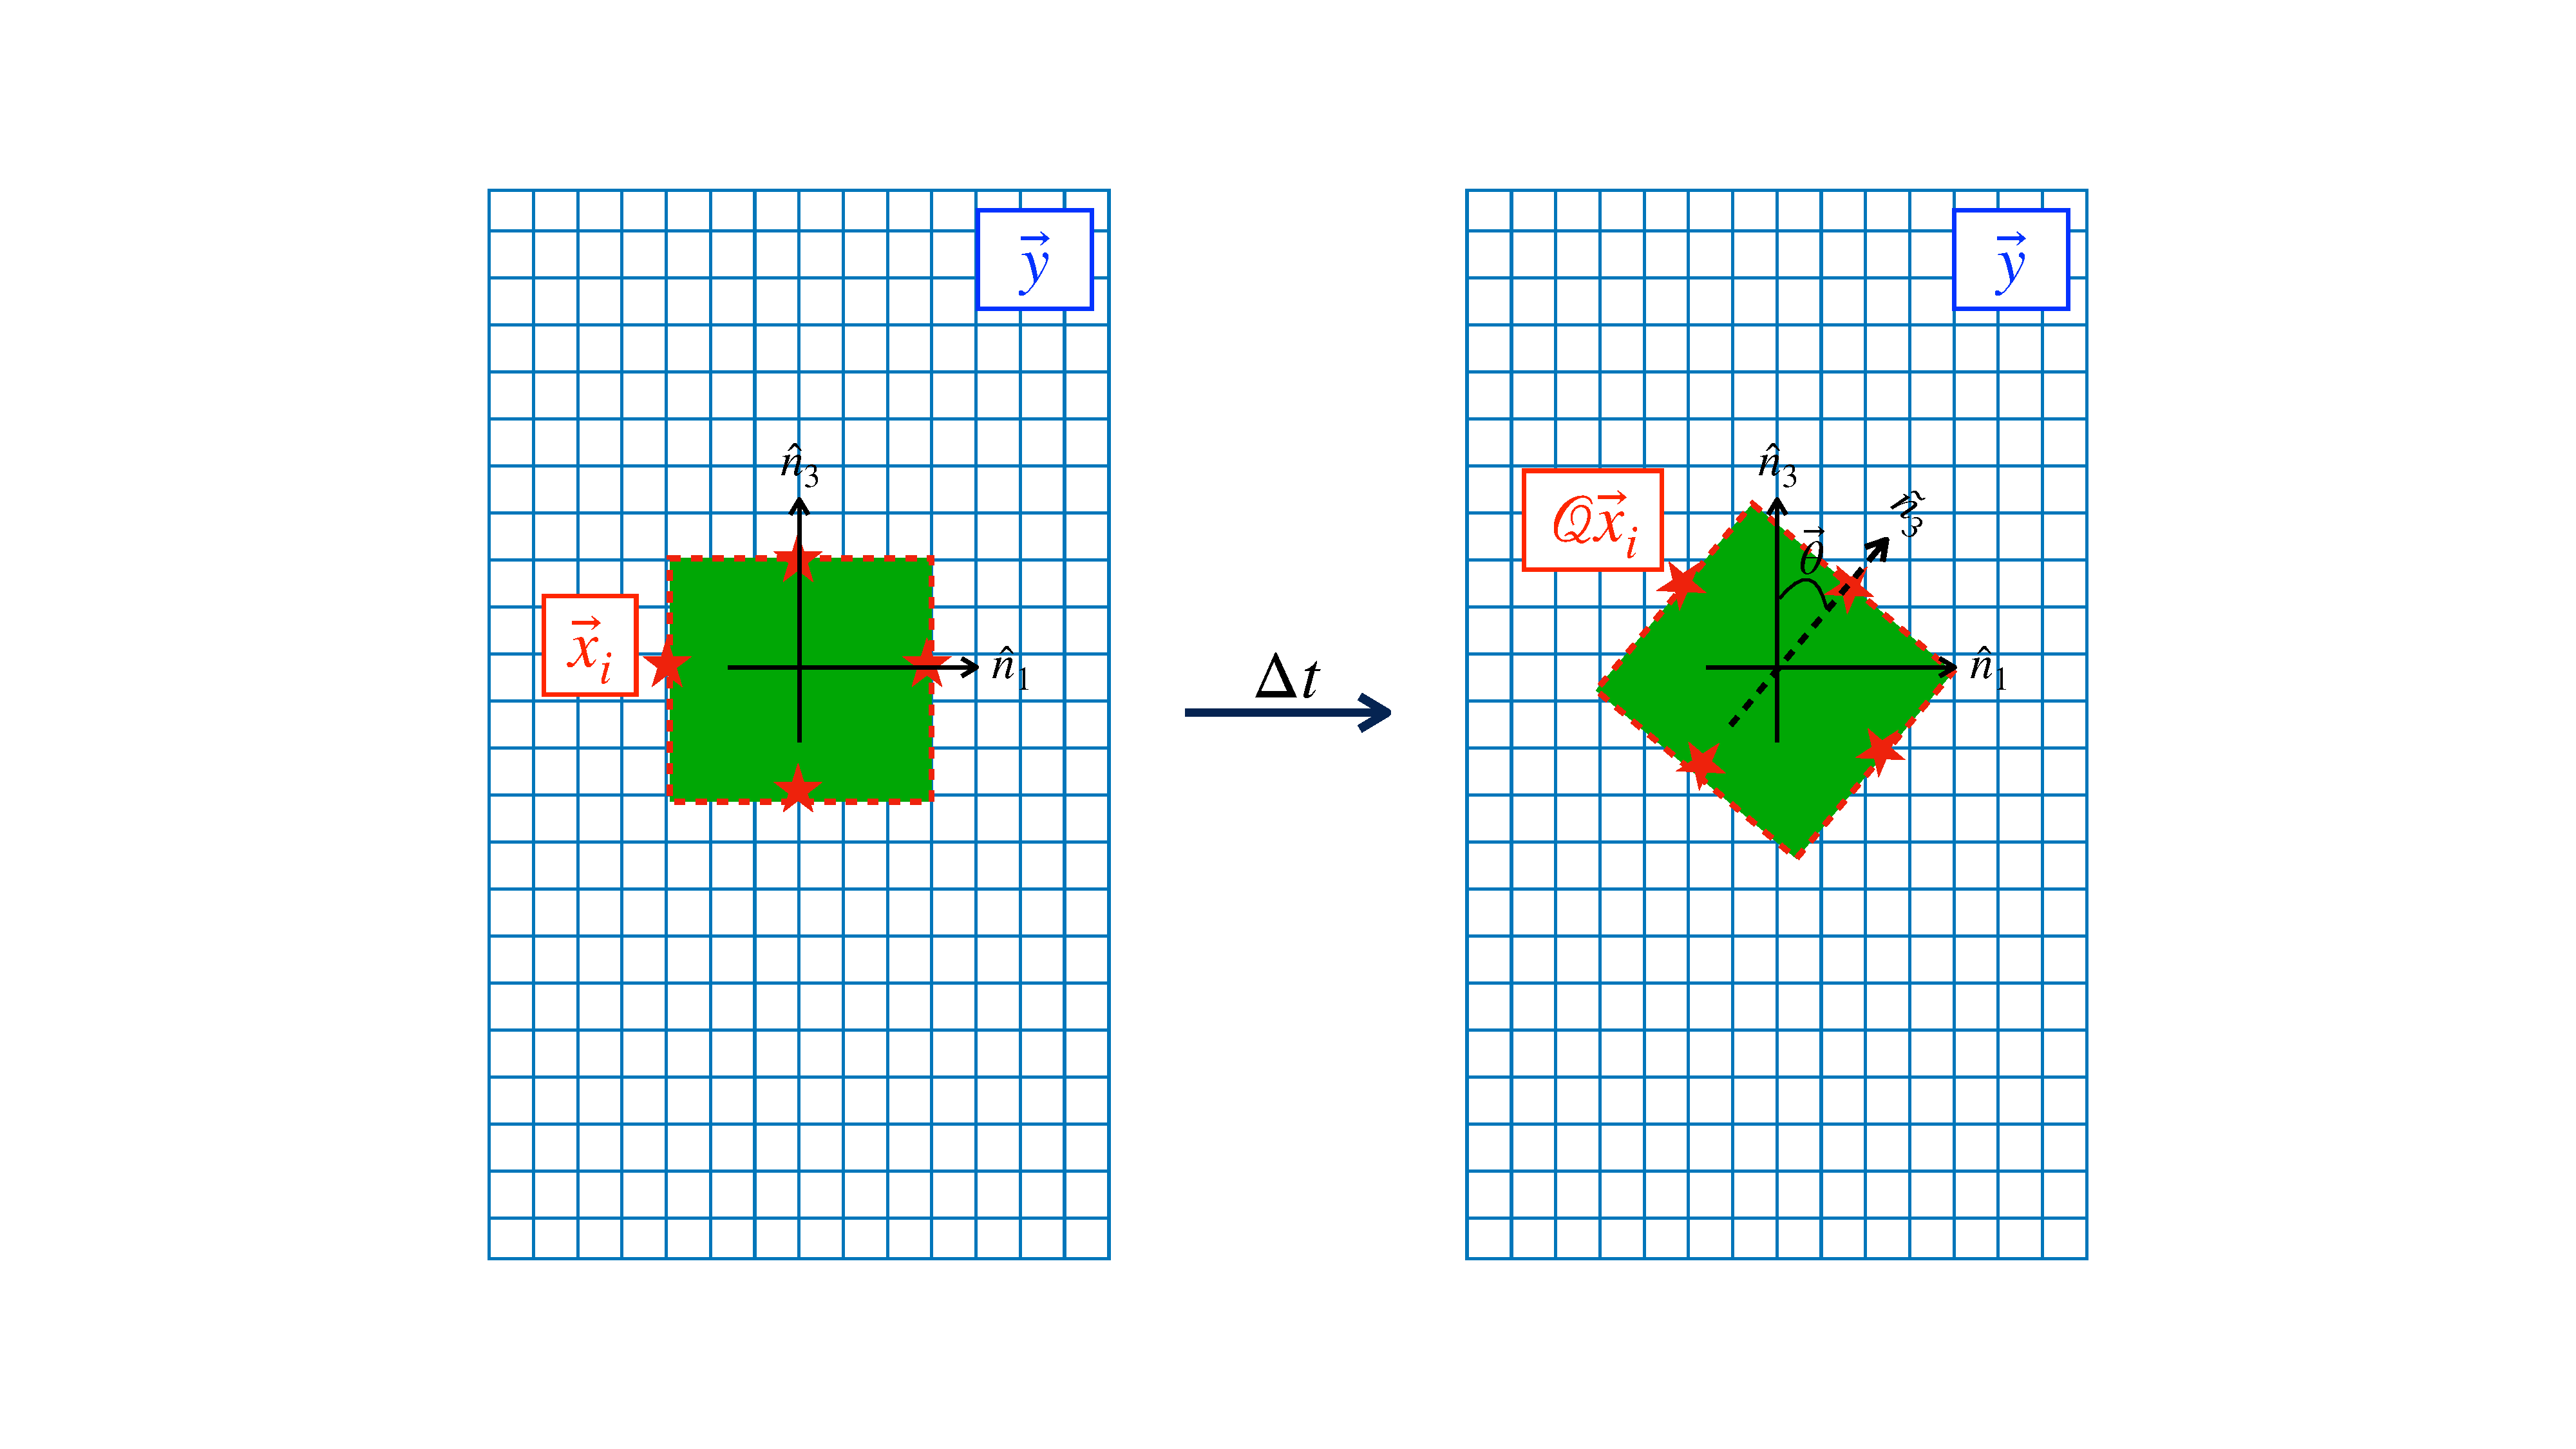
\includegraphics[scale=0.25]{./figures/fig_rotation_schematics.pdf}
	\caption{Schematics of the rotation of an aggregate. The blue grid is the fluid domain and the green rectangle represents an aggregate. Red stars show points on the aggregate.}
	\label{fig_rotation_schematics}
\end{center}
\end{figure}
This information lives in the orientation matrix, $\mathcal{Q}(t)$. We can update our aggregate position from $\vec{x}$ to $\vec{x}_{\mathcal{R}}$ using
\[
\vec{x}_{\mathcal{R}}(t) = \mathcal{Q}(t) \vec{x}.
\]
Note that $\mathcal{Q}(0) = \bar{\bar{I}}$ (identity matrix) at initial time. After we move forward one time step, we may update this orientation matrix as 
\begin{equation}
	\mathcal{Q}(t + \Delta t) = \mathcal{R} \mathcal{Q}(t),
\end{equation} 
where $\mathcal{R}$ is the rotation matrix. 
\par
Assume we obtain the angular velocity, $\vec{\Omega}$ from a time step. (Initially, it is zero vector). With this, we can find the three-dimensional change of angular position vector, $ \vec{\Omega} \Delta t = \left( \Delta \theta_1, \ \Delta \theta_2, \ \Delta \theta_3 \right) \equiv \Delta \vec{\theta}$.
The matrix $\mathcal{A}$ is then defined as 
\begin{equation}
	\mathcal{A}
	=\begin{bmatrix}
	 0 & - \Delta \theta_3 & \Delta \theta_2  \\
	 \Delta \theta_3 & 0  & -\Delta \theta_1  \\
	 - \Delta \theta_2 & \Delta \theta_1 & 0  \\
	\end{bmatrix},
	\label{eq_rotation_mx}
\end{equation}
From here, we have the rotation matrix $\mathcal{R} = e^{\mathcal{A}}.$
We can compute the matrix exponential $e^{\mathcal{A}}$ using Rodrigues' formula,
\begin{equation}
	\mathcal{R} = 
e^{\mathcal{A}} 
 = \bar{\bar{I \ }} 
 + \frac{\sin(\phi)}{\phi} \mathcal{A}
 + \frac{1-\cos(\phi)}{\phi^2} \mathcal{A}^2,
\label{eq_R_eA}
\end{equation} 
where $\phi = \|\Delta \vec{\theta}\|_2$.
With this $\mathcal{R}$ and orientation matrix $\mathcal{Q}$, we are ready to update the fluid grid.


	
\subsection{Linear system in a rotated coordinate}
We first solve for the stress at the center of each square face of an aggregate, $\vec{y} = \vec{x}_i$, 
using the same formula as equation (\ref{eq_vel_all_onS_nonD}),
\begin{equation}
	\vec{u} \left(\vec{x}_i \right) 
		  = -\int_{S}  
		 \vec{f}(\vec{x}) 
		 \cdot \bar{\bar{G \ }} (\vec{x}, \vec{x}_i) 
		 \ \textrm{d}S 
		 - \frac{ \alpha C_{max}}{8\pi } \frac{\rho_0}{(\rho_s - \rho_0)(1-\phi)}
		 \int_V  C \left(\vec{x} ,t \right) \hat{k} \cdot
		 \bar{\bar{G \ }}(\vec{x}, \vec{x}_i)
		 \ \text{d}V,
		 \nonumber
\end{equation}
As we allow rotation, we can express the above equation as
\begin{align}
	\vec{u} \left(\mathcal{Q} \vec{x}_i \right) 
		  = & - \frac{1}{8 \pi} \int_{S}  
		 \vec{f}(\mathcal{Q} \vec{x}) 
		 \cdot \bar{\bar{G \ }} (\mathcal{Q} \vec{x},\mathcal{Q}\vec{x}_i) 
		 \ \textrm{d}S
		 \nonumber \\
		 & - \frac{ \alpha C_{max}}{8\pi } \frac{\rho_0}{(\rho_s - \rho_0)(1-\phi)}
		 \int_V  C \left(\vec{x} ,t \right) \hat{k} \cdot
		 \bar{\bar{G \ }}(\vec{x}, \mathcal{Q} \vec{x}_i)
		 \ \text{d}V.
	\label{eq_slp_On_rotate}
\end{align}
Since the rotation matrix $Q$ is constant and it is normalized, it is valid to say that
\[
 \bar{\bar{G \ }} (\mathcal{Q} \vec{x},\mathcal{Q}\vec{x}_i) 
	 = \bar{\bar{G}}( \vec{x}, \vec{x}_i).
\]
We now solve for unknowns, including the translational and angular velocities,
in a rotated coordinate system $\mathcal{Q} \vec{x}_i $.
Note that the stress values we obtain here 
are located in the same one as the rotated positions.  
To complete the linear system to solve for stress, translational, and angular velocities, we temporarily map the fluid domain grid into the same coordinate system as the boundary integral term.
We can simply muptipliy by $\mathcal{Q}^{-1} = \mathcal{Q}^{T}$ as 
\begin{align}
	\vec{u} \left(\mathcal{Q} \vec{x}_i \right) 
		  & + \frac{1}{8 \pi} \int_{S}  
		 \vec{f}(\mathcal{Q} \vec{x}) 
		 \cdot \bar{\bar{G \ }} (\mathcal{Q} \vec{x},\mathcal{Q}\vec{x}_i) 
		 \ \textrm{d}S
		 \nonumber \\ & =
		 \mathcal{Q}^{-1}
		 \left[
		 - \frac{ \alpha C_{max}}{8\pi } \frac{\rho_0}{(\rho_s - \rho_0)(1-\phi)}
		 \int_V  C \left(\vec{x} ,t \right) \hat{k} \cdot
		 \bar{\bar{G \ }}(\vec{x}, \mathcal{Q} \vec{x}_i)
		 \ \text{d}V
		 \right].
	\label{eq_slp_vol_R}
\end{align}
For the other force equations as well, we implement the following
\begin{equation}
	\int_{S} \vec{f}(\vec{x}) \  \text{d}S(\vec{x})
	= \mathcal{Q}^{-1} \vec{F}_o
	 \label{eq_drag_code}
	 \end{equation} 
	 \begin{equation}
		 \int_S \vec{f} (\vec{x})  \times (\vec{x} - \vec{x}_{cm}) 
		 \ \textrm{d}S(\vec{x}) 
		 = \vec{0}.
	 \label{eq_torque_code}
	 \end{equation}
Once we solve the linear system, we may return the values on the fluid grid to the Cartesian coordinate system.
% We need to rotate them using
% \[
% \vec{f}(\vec{x}_s) = \mathcal{Q} \vec{f}(\vec{x}).	
% \]
% \[
% \vec{U}_a (\vec{x}_s) = \mathcal{Q} \vec{U}_a (\vec{x}).	
% \]
% \[
% \vec{\Omega}(\vec{x}_s) = \mathcal{Q} \vec{\Omega}(\vec{x}).	
% \]
% The validation of stress is in section (\ref{validation_rot}).
\subsection{Velocity compuation}
Once we solve for the stress, we are supposed to use the same 
equation (\ref{eq_vel_all_onS_nonD}) 
to solve for velocity in the fluid grid, which stays in the Cartesian coordinates.
Although the volume integral term can stay as it is,  
the boundary integral needs some special treatment
since it has two mixed coordinate systems.
We particularly pay more attention to the Stokeslet,
\[
	\bar{\bar{G \ }} (\mathcal{Q}\vec{x},\vec{y}) 
	= 
	\frac{\bar{\bar{I \ }}}{||\mathcal{Q}\vec{x}-\vec{y} ||} 
	+ \frac{(\mathcal{Q}\vec{x}-\vec{y})(\mathcal{Q}\vec{x}-\vec{y})^T}{||\mathcal{Q}\vec{x}-\vec{y} ||^3}, 	 
\]
where $\mathcal{Q}\vec{x}$ is in the aggregate rotated grid. Since we cannot compute the boundary integral of the Stokeslet when $\mathcal{Q}\vec{x}$ and $\vec{y}$ are not in the same coordinate system, we need to express $\vec{y}$ using another vector $\vec{v}$ that is in the rotated grid such that 
\[
	\mathcal{Q}\vec{x} - \vec{y} = \vec{x} - \vec{v},
	% \mathcal{Q}\vec{x}-\vec{v} = \vec{x} - \vec{y},
\]
or equivalently,
\[
	\vec{v} = \left(   \bar{\bar{I}} - \mathcal{Q} \right) \vec{x}  + \vec{y}.
\]
% {\color{blue} Need to type below figure.}
% \begin{figure}[h]
% 	\begin{center}
% 		\includegraphics[scale=0.45]{./figures/fig_vel_y_map}		
% 		\caption{Mapping for $\vec{y}$ grid.}
% 		\label{fig_vel_y_map}
% \end{center}
% \end{figure}

After we solve for the velocity field of the fluid domain, we rotate the velocity field back to the original coordinate by multiplying by the inverse of $\mathcal{Q}$ for the concentration update. 
%---------------Numerics--------------------------------------
\section{Numerical methods}
%---------------------------------------------------------
% {\color{blue} NEED TO EDIT MORE OF THE BEGINNING OF THIS SECTION $\downarrow$}\\
% As we have stratified density in the surrounding fluid, 
% numerical methods for the homogeneous solution, that is, the BIE computation, was explained in section \ref{sec:numerical}. For the advection-diffusion equation, it is described in section \ref{sec:concentration}.

We first consider the background fluid density that is a part of the drag computation. We derive the simplest form to implement in codes. We then discuss the homogeneous velocity field. We briefly introduce the linear system to solve for the aggregate's stress and velocity. Lastly, we present the method to compute the non-homogeneous solution, a volume integral of the perturbation $C(\vec{x},t)$. Due to the high computational cost, we use the fast multipole method (FMM). We briefly introduce the FMM and framework for the Stokes kernel.
 \subsection{Aggregate force balance}
Since the surrounding fluid density is not constant while an aggregate settle, we need to track the buoyancy depending on the aggregate's vertical position,
\begin{align}
	\vec{F}_{b}
	 = \frac{1}{\tilde{\mu} U_s R_a} 
	 \left(
	  \int_{S} \left( 
	  \int \rho_{bg}(z) g \ \textrm{d}z 
	  \right) \bar{\bar{I \ }}  \cdot
	 \hat{n} \ \textrm{d}S (\vec{x})
   \right).
   \label{eq_buoyancy_nonD}
\end{align}
Furthermore, the fluid density portion of the aggregate changes over time, which also affects its gravitational (body) force,
\begin{equation}
	\vec{F}_g = 
	- \frac{1}{\tilde{\mu} U_s R_a} 
	\left( \rho_a V_a g \hat{k}	 \right).
	\label{eq_agg_force_G}
\end{equation}
Evaluating the gravitational force (\ref{eq_agg_force_G}) is relatively easy in practice. While settling, we compute the fluid density where the aggregate is located. Once we know the fluid grid point inside the aggregate, simply adding the densities at those points gives us the fluid density portion of the aggregate, which eventually plays a role in updating the $\rho_a$. 

\par
Next, we investigate the buoyancy force (\ref{eq_buoyancy_nonD}) with a single cube case for simplicity. 
We can extend this case to multiple cubes in the same manner by addition. We consider the discretized version of integral (\ref{eq_buoyancy_nonD}), 
\begin{equation}
	\vec{F}_b \approx
	\frac{1}{\tilde{\mu} U_s R_a} 
	\sum_{i=1}^{N_f}
	 R_a^3 \int_{S^i} \left( 
	   \int  {\rho_{bg}} (z) g  \ \textrm{d}z 
	 \right) \bar{\bar{I \ }}  \cdot
	\hat{n}_i \ \textrm{d}S^i (\vec{x}),
\label{eq_buoyancy_discrete2}
\end{equation}
where $i$ represents the index of square faces (not power), and $N_f$ is the number of square faces: $N_f = 6$ for one cube case. Depending on the orientation of each square face, or the axis of $S^n$, is different. For example, let $S^1$ be the first square with the normal $\hat{n}_1 = (1,0,0)$, i.e., 
\begin{equation}
	R_a^3 
	 \int_{S^1}
	 \left( 
	   \int  {\rho_{bg}} (z) g \ \textrm{d}z 
	 \right) \bar{\bar{I \ }}  \cdot
	\hat{n}_1 \ \textrm{d}S^1 (\vec{x})
	= R_a^3  \int_{-1}^{1} \int_{-1}^{1}
	\left( 
  	 \int  {\rho_{bg}} (z) g \ \textrm{d}z 
 	\right) \bar{\bar{I \ }}  \cdot
 	\hat{n}_1 \ 
	\textrm{d}y  \textrm{d}z.
\label{eq_buoyancy_S1_2}
\end{equation}
See Figure \ref{fig_rho_bg_on_S1} for notations.
\begin{figure}[h]
	\begin{center}
		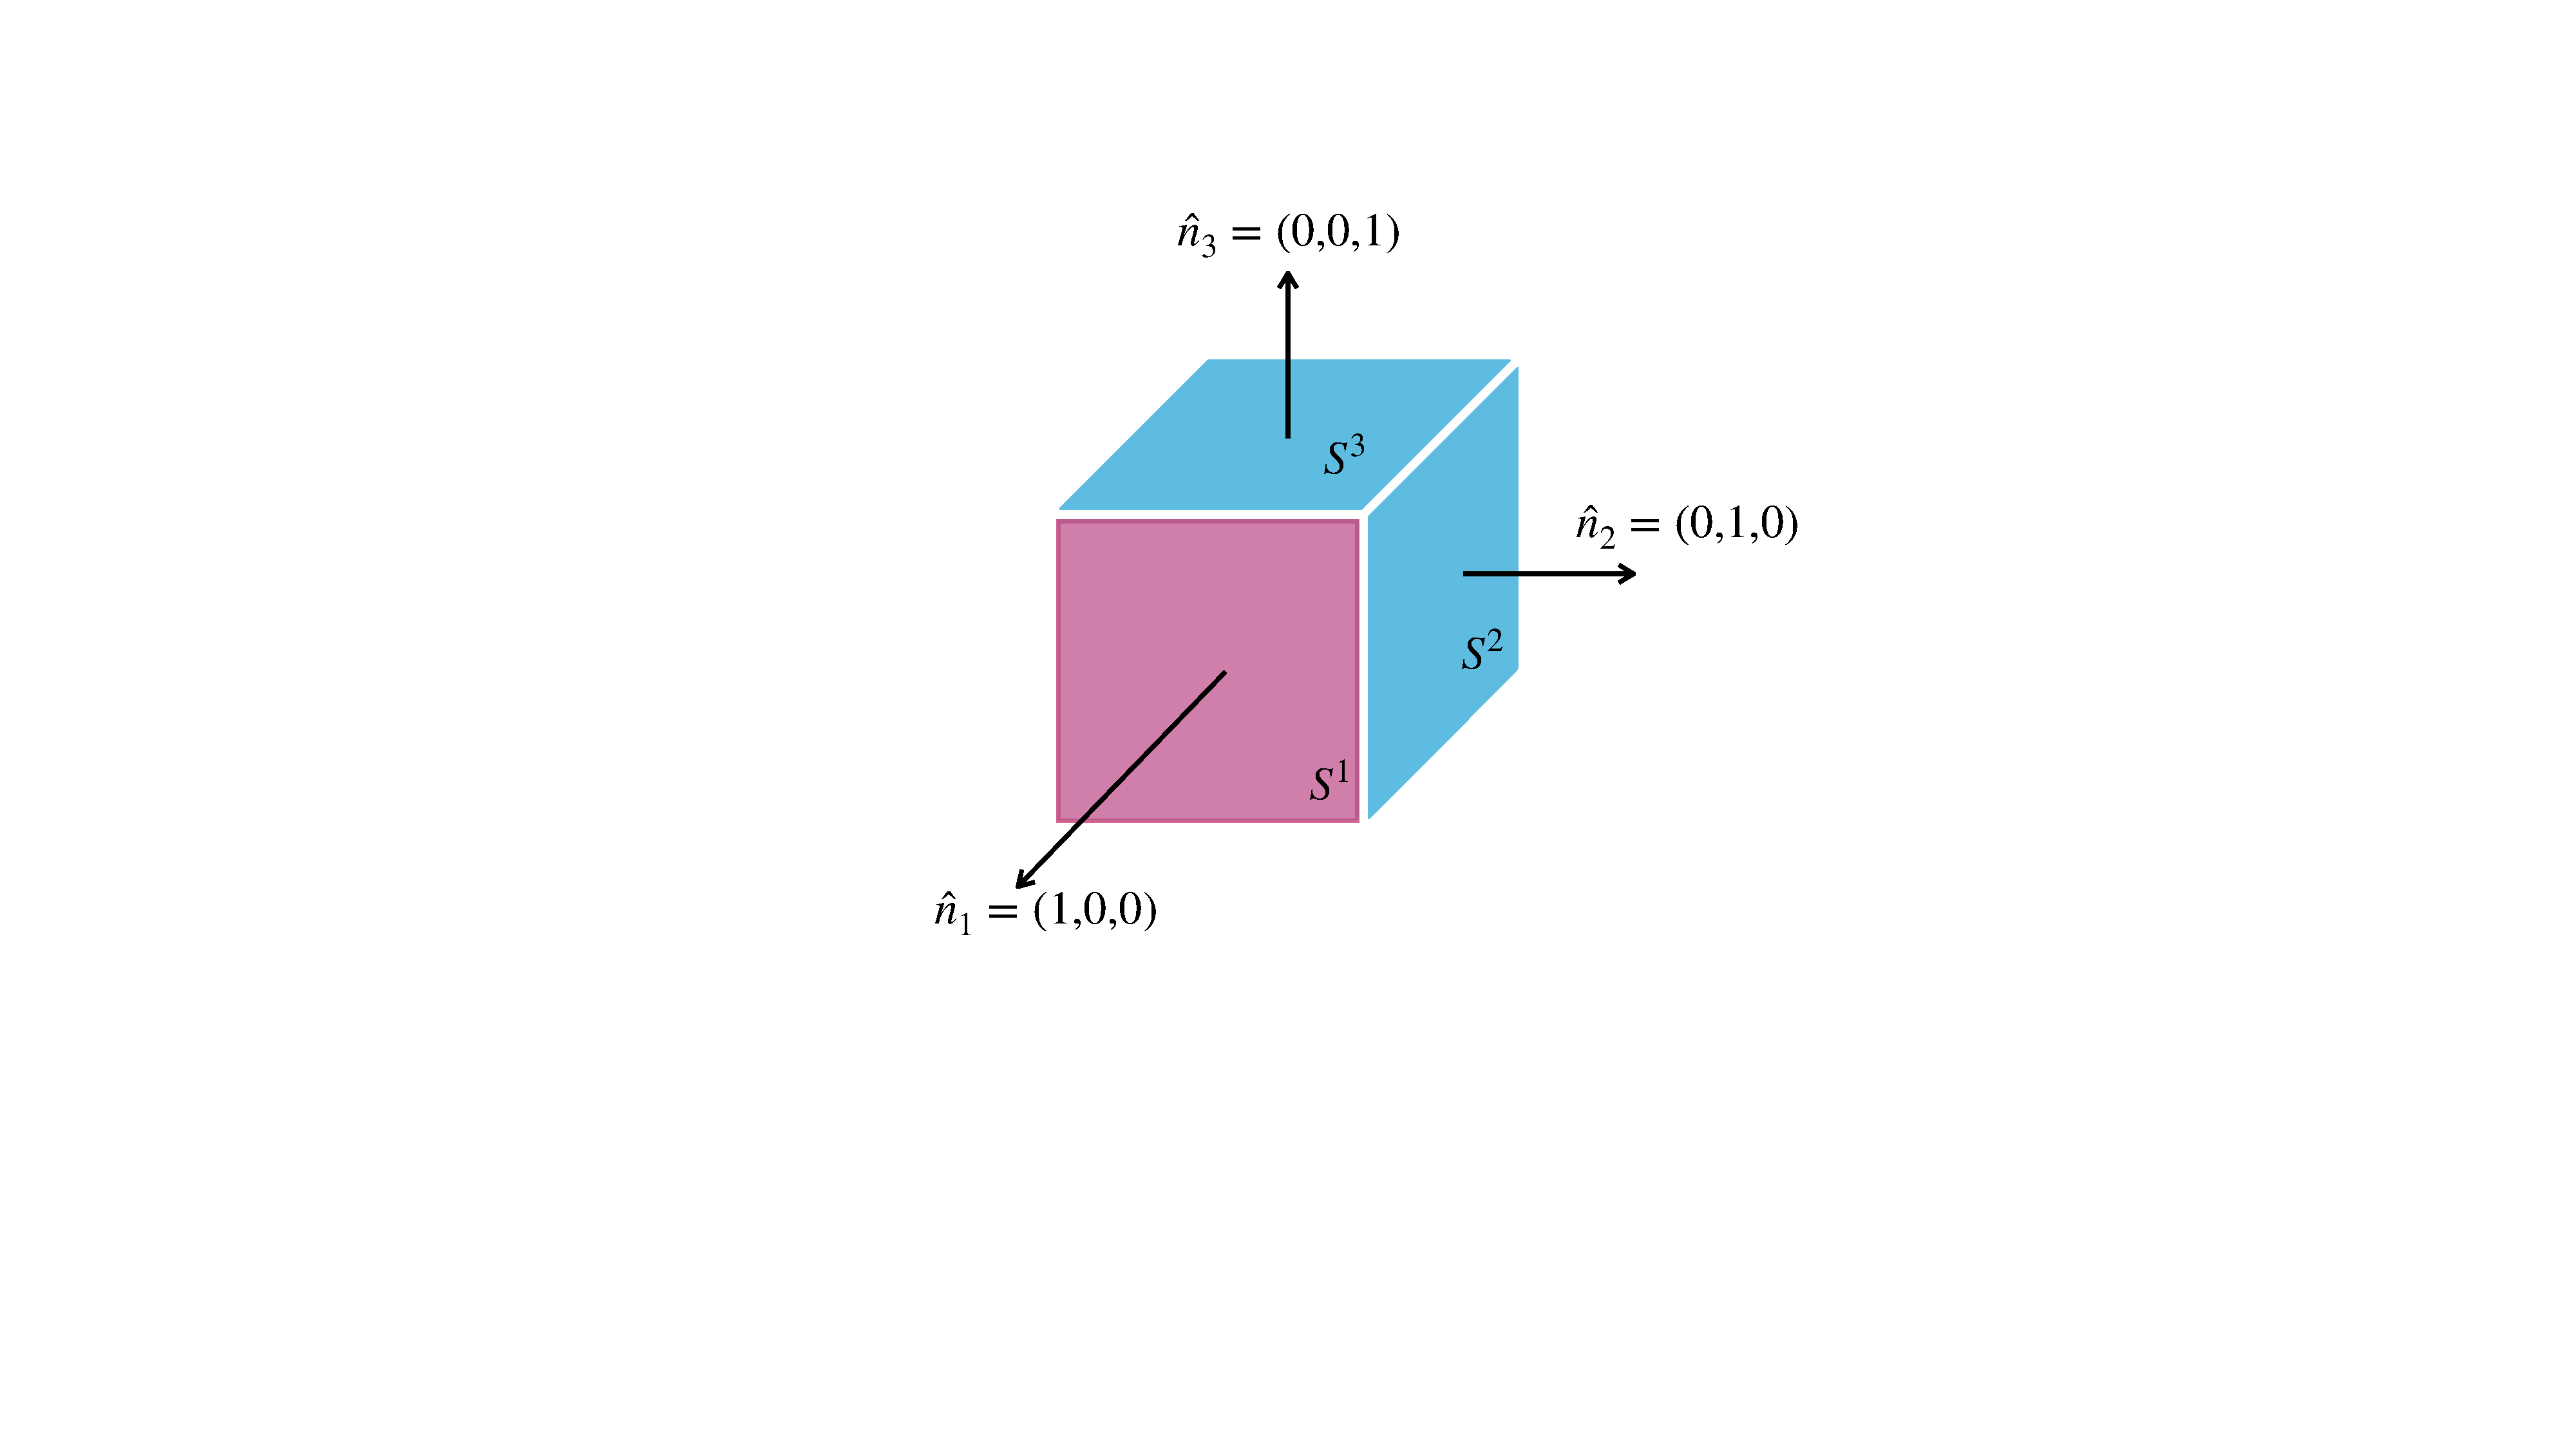
\includegraphics[scale=0.3]{./figures/fig_rho_bg_on_S1.pdf}
	\caption{Example cube to describe the buoyancy force computation. The pink area is $S^1$ integral domain.}
	\label{fig_rho_bg_on_S1}
\end{center}
\end{figure}
Since the background density $\rho_{bg}$ is a function of $z$-axis only, we can intuitively see that the value (\ref{eq_buoyancy_S1_2}) and the one with the normal $\hat{n}_6 = -\hat{n}_1 = (-1,0,0)$ has the same magnitude but in the opposite direction. It means the sum of integrals on the planes $S^1$ and $S^6$ is zero. We can also prove this with simple arithmetics. 
We first write the inner integral explicitly using equation (\ref{eq_rho_bg}),
\[
R_a^3 \int  {\rho_{bg}} (z)g  \ \textrm{d}z 
 =  R_a^3 \left( \rho_0 \int  1+\gamma  z \right) g \ \textrm{d}z 
=R_a^3 \rho_0 \left(  z + \frac{\gamma}{2}z^2 + c \right) g,
\]
where $c$ is an integral constant. 
% This form is valid for any $z$. 
The surface integral on $S^1$ then becomes 
\begin{equation}
	R_a^3\rho_0  \int_{-1}^{1} \int_{-1}^{1}
	\left( 
	 z + \frac{\gamma}{2}z^2 + c 
   \right) g \bar{\bar{I \ }}  \cdot
   \hat{n}_1 \ 
  \textrm{d}y  \textrm{d}z 
=4 R_a^3 \rho_0 \left( c + \frac{\gamma}{6} \right) g \hat{n}_1 .
\label{eq_F_by_S1}
\end{equation}
We notice that we can obtain the same integral value as equation (\ref{eq_F_by_S1}) on $S^6$, as well as  $S^2$ and $S^5$, in which their normals are $\hat{n}_2 = -\hat{n}_5 = (0,1,0)$. It implies that we have 
\begin{equation}
	\sum_{i=1,2,5,6}
	 R_a^3 \int_{S^i} \left( 
	   \int  {\rho_{bg}} (z) g  \ \textrm{d}z 
	 \right) \bar{\bar{I \ }}  \cdot
	\hat{n}_i \ \textrm{d}S^i (\vec{x})
	 = 0
\label{eq_buoyancy_zero_oneCube}
\end{equation}
for the one cube case of discretized buoyancy equation (\ref{eq_buoyancy_discrete2}).
\par
The integrals on $S^3$ and $S^4$ are slightly different since the square faces are perpendicular to $z-$axis. On the face $S^3$, which has normal $\hat{n}_3 = (0,0,1)$, we get
\begin{equation}
	R_a^3
\rho_0\int_{-1}^{1} \int_{-1}^{1}
  	\left( 
  	 z + \frac{\gamma}{2}{z}^2 + c 
 	\right)g  \bar{\bar{I \ }}  \cdot
 	\hat{n}_3 \ 
	\textrm{d}x  \textrm{d}y 
	= 4 R_a^3 \rho_0 \left( z_T + \frac{\gamma}{2} {z_T}^{2} +c \right) g \hat{n}_3,
	\label{eq_F_by_S3}
\end{equation} 
where $z_T$ is the constant $z-$level value on the face $S^3$. The integral value on the face $S^4$ would be the same as \ref{eq_F_by_S3}, having $\hat{n}_4 = (0,0,-1)$ instead of $\hat{n}_3$. We then can have a more explicit expression for the discretized buoyancy equation (\ref{eq_buoyancy_discrete2}),
\begin{align}
	\sum_{i=1}^{6} R_a^3
	 \int_{S^i} \left( 
	   \int  {\rho_{bg}} (z)  \ \textrm{d}z 
	 \right) g \bar{\bar{I \ }}  \cdot
	\hat{n}_i \ \textrm{d}S^i (\vec{x})
	\nonumber 
	\\
	= 4 R_a^3 \rho_0 \left( z_T + \frac{\gamma}{2} {z_T}^{2} +c \right) g \hat{n}_3
	+ 4R_a^3 \rho_0 \left( z_B + \frac{\gamma}{2} {z_B}^{2} + c \right) g \hat{n}_4,
\label{eq_buoyancy_discrete_eval2}
\end{align}
where $z_B$ is the constant $z-$ value of the surface $S^4$ (bottom face). By substituting the normals $\hat{n}_3$ and $\hat{n}_4$, we can simplify the right-hand side of equation (\ref{eq_buoyancy_discrete_eval2}), knowing that $z_T - z_B = 2$, the equation (\ref{eq_buoyancy_discrete_eval2}) becomes 
\begin{equation}
	\sum_{i=1}^{6} R_a^3
	\int_{S^i} \left( 
	  \int  {\rho_{bg}} (z)  \ \textrm{d}z 
	\right) g \bar{\bar{I \ }}  \cdot
   \hat{n}_i \ \textrm{d}S^i (\vec{x})
= 8 R_a^3 \rho_0 \left( 1+ \gamma z_{c_n} \right) g, 
\label{eq_buoyancy_z_eval2}
\end{equation}
where we define the $z-$component of the center of $n-$th cube forming an aggregate, $z_{c_n}$ ($ n = 1, 2, \cdots, $NC).
We thus have shown that the only information we need to keep track of is the location of the center of each cube that forms an aggregate.
%
 \subsection{Linear system for velocity and stress on aggregates}
 As mentioned above, we do not prescribe the settling velocity of an aggregate, and it becomes unknown.
We thus need to solve for 1) translational velocity ($\vec{U}_a$), 2) rotational velocity ($\vec{\Omega}$), and 3) stress vector ($\vec{f}$).
To do so, 
we build the system using equations (\ref{eq_Fo}), (\ref{eq_Qo}), and the velocity combine with equations (\ref{eq_vel_all_onS_nonD}) and (\ref{eq_solidbody}), that is,
 \begin{align}
	\vec{U}_a + \vec{\Omega} \times (\vec{x} - \vec{x}_{cm})
+ \frac{1}{8 \pi} \int_{S}  
		  \vec{f}(\vec{x}) 
		  \cdot \bar{\bar{G  }} (\vec{x},\vec{y}) 
		  \ \textrm{d}S(\vec{x})
		  \nonumber \\
=  -\frac{ \alpha C_{max}}{8\pi } \frac{\rho_0}{(\rho_s - \rho_0)(1-\phi)} 
\int_{V} C\left(\vec{x},  t \right) \hat{k} \cdot 
\bar{\bar{G}}(\vec{x}, \vec{y} ) 
\ \text{d}V(\vec{x}),
 \label{eq_slp_lin_eq}
 \end{align}
where the volume integral value on the right-hand side is known. 
To set up the linear system accordingly, We discretize the boundary integral as described in the equation (\ref{eq_discretized}), choosing $\vec{f}_k$ for $\vec{q}_k$, and $ \bar{\bar{G}}$ for $\bar{\bar{J}}$, 
\begin{equation}
	\vec{I}(\vec{x}_{sq,i})  =   \sum_{k=1}^{N_f}  \vec{f}_k   \int_{S_{k}} \bar{\bar{G}}(\vec{x},\vec{x}_{sq,i}) \ \text{d}S(\vec{x}) 
	= \sum_{k=1}^{N_f} \vec{f}_k   \ \bar{\bar{\Pi}}_{i,k}
	\approx \int_{S}  
	\vec{f}(\vec{x}) 
	\cdot \bar{\bar{G  }} (\vec{x},\vec{y}) 
	\ \textrm{d}S(\vec{x}).
\end{equation}
The exact linear system of the equations (\ref{eq_slp_lin_eq}),  (\ref{eq_Fo}), and (\ref{eq_Qo}) we implement is  
 \begin{align}
	\tiny
		%---A------------------------------------------------------------
 	\left[
 	    \begin{array}{c;{2pt/2pt}c; {2pt/2pt}c}
 			\phantom{,} & \phantom{,}& \phantom{,}
 			\\
		   \begin{bmatrix}
 				\bar{\bar{\Pi}}_{1,1} & 
 				\bar{\bar{\Pi}}_{1,2} &
 				\cdots & \bar{\bar{\Pi}}_{1,N_f}
 				\\
 				\\
 				\bar{\bar{\Pi}}_{2,1} & 
 				\bar{\bar{\Pi}}_{2,2} &
 				\cdots & \bar{\bar{\Pi}}_{2,N_f}
 				\\ 
 				\vdots &  \vdots & \ddots & \vdots
 				\\
 				\\
 				\bar{\bar{\Pi}}_{N_f,1}&
 				\bar{\bar{\Pi}}_{N_f,2} &
 				 \cdots & \bar{\bar{\Pi}}_{N_f,N_f}
 		\end{bmatrix}
 			 & 
 			 \begin{bmatrix}
 				 \bar{\bar{I \ }}
 				 \\
 				 \vdots
 				 \\
 				 \\
 				  \bar{\bar{I \ }}
 			\end{bmatrix}
 			  & -
    			 \begin{bmatrix}
    				  [\vec{x}_{sq,1} - \vec{x}_{cm}]_{\times}
    				 \\
    				 \vdots
    				 \\
    				 \\
    				   [\vec{x}_{sq,N_f} - \vec{x}_{cm}]_{\times}
    			\end{bmatrix}
 			\\
 			\phantom{,} &\phantom{,} &\phantom{,}
 			\\
 			\hdashline[2pt/2pt]
 			\phantom{,} &\phantom{,} &\phantom{,}
 			\\
 			 \begin{bmatrix}
 				 \bar{\bar{I \ }}
 				 &
 				 \cdots
 				 &
 				  \bar{\bar{I \ }}
 			\end{bmatrix}
 			&  \bar{\bar{0}}  & \bar{\bar{0}}
 			\\
 			\phantom{,} &\phantom{,} &\phantom{,}
 			\\
 			 \hdashline[2pt/2pt]
 			 \phantom{,} &\phantom{,} &\phantom{,}
 			\\
 			 - \begin{bmatrix}
 				[\vec{x}_{sq,1} - \vec{x}_{cm}]_{\times}
 				 &
 				 \cdots
 				 &
 				  [\vec{x}_{sq,N_f} - \vec{x}_{cm}]_{\times}
 			\end{bmatrix}
 			& \bar{\bar{0}}  &  \bar{\bar{0}}
  	 	\\
 			\phantom{,} & \phantom{,}& \phantom{,}
 	    \end{array}
 	\right]
 	%---x------------------------------------------------------------
 	\left[
 	\begin{array}{c}
 		\vec{f}_1
 		\\ \\
 		\vdots \\
 		\\
 		\vec{f}_{N_f}
 		 \\ \\  \hdashline[2pt/2pt]
 		\\
 		 \vec{U}_a
 	  	\\
 	 	\\
 	 	\hdashline[2pt/2pt]
 	 	\\
 	 	\vec{\Omega}
 	\end{array}
 	\right]
 		%---b------------------------------------------------------------
 	=
 	\left[
 	\begin{array}{c}
 		{\vec{\mathcal{F}}}^1  \\ \\
 		\vdots \\
 		\\
 		{\vec{\mathcal{F}}}^{N_f} \\ \\  \hdashline[2pt/2pt]
 		\\
 		 \frac{1}{4}\vec{F}_o
 	  	\\
 	 	\\
 	 	\hdashline[2pt/2pt]
 	 	\\
 	 	\frac{1}{4}\vec{Q}_o
 	\end{array}
 	\right].
 \label{eq_slp_linear_system}
 \end{align}
 Since we consider three-dimensional space, the size of the identity matrix $\bar{\bar{I}}$ is $(3 \times 3)$. The matrix $[\vec{y}]_{\times}$ represents the cross product operator defined by,
 \begin{equation}
 	[\vec{y}]_{\times} = \begin{bmatrix}
 	0 & -y_3  & y_2 \\ 
 	 y_3 & 0  & -y_1\\ 
 	- y_2 & y_1  & 0
 	\end{bmatrix},
 	\label{eq_cross_2}
 \end{equation}
 where $\vec{y} = (y_1, y_2, y_3).$
We use this operator for the rotation term, 
 \[
  [\vec{x} - \vec{x}_{cm}]_{\times}  \vec{\Omega}
   = (\vec{x} - \vec{x}_{cm}) \times \vec{\Omega}
  = - \vec{\Omega} \times  (\vec{x} - \vec{x}_{cm}),
  \]
  in the total torque equation.
In addition, the top part of right-hand side of the equation (\ref{eq_slp_lin_eq}) represents 
\begin{equation}
	{\vec{\mathcal{F}}} (\vec{x}_{sq,i}) = 
	-\frac{ \alpha C_{max}}{8\pi } \frac{\rho_0}{(\rho_s - \rho_0)(1-\phi)} 
   \sum_{j= 1}^{Ns}  C \left(\vec{x}_{sq,i},  t \right) \hat{k} \cdot
   \bar{\bar{G \ }}(\vec{x}_{sq, i}, \vec{x}_{j} ),
\label{eq_volume_rhs}
\end{equation}
   where $Ns$ is the total number of grid or source points in the fluid domain. We discuss more details of the volume integral computation in the next section. 
%    \ref{section_volume_int}.
  One can find the factor 1/4 multiplied by the second and third blocks on the right-hand side of the system (\ref{eq_slp_linear_system}). 
 Since we set the side length of a cube as 2, factor 4 represents the area of a square face that is the integral domain of the total force and torque equations. 
 \par
 Once we invert the linear system and obtain the unknowns, we use the equation (\ref{eq_vel_all_onS_nonD}) to calculate the velocity field at all points in the fluid domain. We want to point out that the fluid velocity computation, especially including the volume integral (\ref{eq_volume_rhs}), is a very numerically expensive job. To accelerate it, we apply the fast multipole method (FMM) to our simulations. In the following section, we explain how we use the FMM. 
\subsection{Fast Multipole Method (FMM)}
Knowing that we simulate our problem in a three-dimensional fluid domain, it is necessary to implement an efficient and fast method for each part of the codes while we keep the stability and desired accuracy. 
The FMM is a numerical scheme for rapid computation of $N$-body problems governed by a Green's function using a multipole expansion. It was first introduced by Greengard and Rokhlin \cite{greengard_fast_1987}. Since then, the researchers at Flatiron Institute - Simons Foundation,  including
the original authors of the FMM, have developed the methods and shared the source code. We choose to use their library, called \href{https://github.com/flatironinstitute/FMM3D}{{\color{blue}FMM3D}}. It provides the code of the $N-$body interactions governed by Laplace and Helmholtz equations in three-dimension.
For our problem, we can modify the Laplace kernel, as shown in \cite{tornberg_fast_2008}, to compute the integrals of Stokeslet (\ref{eq_stokeslet}).
The definition of Laplace FMM in the FMM3D library is the following:
\begin{definition} (\textit{Laplace FMM})
	\label{eq_def_FMM}
	Let $c^n \in \mathbb{R}$ denote a collection of charge strengths and $\vec{v}^n \in \mathbb{R}^3$ denote a collection of dipole strengths for $n = 1,2, \cdots, N$.
	The Laplace FMM computes the potential $u(\vec{y}^m) \in \mathbb{R}^3$ given by
\begin{equation}
	u(\vec{y}^m) = \sum_{n = 1}^{N} 
		\Biggl[
		\frac{c^n}{\|\vec{x}^n - \vec{y}^m \|}
			- \vec{v}^n \cdot \nabla_{\vec{y}} 
			 \frac{1}{\|\vec{x}^n - \vec{y}^m \|}
		\Biggr],
\label{eq_fmm3d_package}
\end{equation}
	at the \textit{source} ($\vec{x}^n$) and \textit{target} locations ($\vec{y}^m$). 
	% Here, the denominator $\|x_i^n - y_j^m \| = \|\vec{x}^n - \vec{y}^m \|$.
	When $\vec{y}^m = \vec{x}^n$, the term corresponding to $\vec{x}^n$
	is dropped from the sum.
\end{definition}
\noindent
Note that we use the indices $m$ and $n$ to represent the number of target and source points, respectively. For our problem, the points where we want to obtain velocity would be the targets; all points in an integral domain are sources.
In addition to the target and source points, we can input the constant $c^n$ and vector $\vec{v}^{n}$. One needs to be careful about these terms; Both values could depend on the sources but are independent of the targets. 
\subsubsection{Volume integral with the perturbation $C$}
We first investigate how to incorporate the volume integral (\ref{eq_volume_rhs}) (without the prefactor) in the definition (\ref{eq_fmm3d_package}). For a fixed $j$, we can rewrite the equation using the index notation ($i, j = 1,2,3$), 
\begin{equation}
	\tilde{V}(y_j^m)
	\equiv
	 d\sum_{n = 1}^{Ns} \sum_{i = 1}^{3}
	 C(x^n_i,  t)\hat{k} G_{ij}(x_i^n,y_j^m),
	\label{eq_Vn}
\end{equation}
where $\vec{y}^m = (y_1^m, \ y_2^m, \ y_3^m)$ is the target point, $\vec{x}^n = (x_1^n, \ x_2^n, \ x_3^n)$ is the source or grid point in the fluid domain $V$, and $d$ is constant from a quadrature method.
Note that we can use the FMM3D only for points $\vec{y}^m \neq \vec{x}^n \in V$. 
At a singularity, we use MATLAB built-in function, \verb+integral3+, to integrate numerically by defining a small cube $V_p$ around the singularity point,
\begin{equation}
	\mathbb{V}_p(\vec{y}) = 
	 \int_{{V}_p}
		C (\vec{x},t ) \hat{k} \cdot 
		\bar{\bar{G \ }} (\vec{x}, \vec{y} ) 
		\ \text{d}V(\vec{x}).
		\label{eq_vol_int_singular}
	\end{equation}
% where
% 	\[\tiny
% 	V_p = [x_1 - \Delta x_1/2, \ x_1 + \Delta x_1/2]
% 	\times [x_2 - \Delta x_2/2, \ x_2 + \Delta x_2/2]
% 	\times [x_3 - \Delta x_3/2, \ x_3 + \Delta x_3/2].
% 	\]
The Stokeslet can be expressed in terms of the Laplace kernel, $\Phi(\vec{x},\vec{y}) = 1/{\| \vec{x} - \vec{y} \|}$,
\begin{equation}
	G_{ij}(x_i^n,y_j^m)
	 =  \delta_{ij} \Phi \left( x_i^n - y_j^m \right)
	 - \left( x_i^n - y_j^m \right)
	 \frac{\partial}{\partial  x_j}
	\Phi \left( x_i^n - y_j^m \right)
	\label{eq_Gij}
\end{equation}
% Then the inner summation of equation (\ref{eq_Vn}) becomes
% \begin{align*}
%  \sum_{i = 1}^{3}
%  C(x^n_i,  t)\hat{k} G_{ij}(x_i^n,\vec{y}^m)
%  	=  \sum_{i = 1}^{3} C(x^n_i,  t)\hat{k}
% 	\left(
% 	\frac{\delta_{ij}}{\|x_i^n - y_j^m \|}
% 	- \left( x_i^n - y_i^m \right)
% 	 \frac{\partial}{\partial x_j}
% 	\frac{1}{\|x_i^n - y_j^m \|}
% 	\right)
% \end{align*}
By substituting the Stokeslet (\ref{eq_Gij}) into the discretized volume integral (\ref{eq_Vn}), we then get
\begin{equation}
	\tilde{V}_j (\vec{y}^m)=
	\sum_{n=1}^{Ns}
	d
   \sum_{i = 1}^{3} C(x^n_i,  t)\hat{k}
  	\left(
  	\frac{\delta_{ij}}{\|x_i^n - y_j^m \|}
  	- \left( x_i^n - y_j^m \right)
  	 \frac{\partial}{\partial x_j}
  	\frac{1}{\|x_i^n - y_j^m \|}
  	\right)
 \label{eq_frm_lplc_stokes}
\end{equation}
Knowing that the vector $\hat{k} = (0, \ 0, \ 1)$, only $i = 3$ terms survive. We thus reach the simplified sum (\ref{eq_frm_lplc_stokes}),

\begin{align}
	\tilde{V}_j (\vec{y}^m) 
	& = \sum_{n=1}^{Ns} 
		d \ {C}(x_3^n, t)
		\left(
			\frac{ \delta_{3j} }{\|x_3^n - y_j^m \|}
			- 
			 x_3^n  
			\frac{\partial}{\partial x_j}
				\frac{1}{\|x_3^n - y_j^m \|}
				\right)
			\label{eq_vol_target} \\
			& +
			   y_j^m  
			\sum_{n=1}^{Ns} 
			d \ {C}(x_3^n, t)
			\frac{\partial}{\partial x_j}
				\frac{1}{\|x_3^n - y_j^m \|}.
\label{eq_vol_source}
\end{align}
We split the gradient term into two parts since the nature of $x_3^n$ and $y_j^m$ differs. We see that $x_3^n$ is related to the source point as the FMM3D package does. However, $y_j^m$ is the target. 
% We thus need to use the library twice to compute $\tilde{V}_j (\vec{y}^m) $.
The main advantage of this method is that we need to call this Laplace FMM code only once for multiple targets and $N$ number of source points. 
Note that the FMM3D package returns a scalar value. Meanwhile, our summation has a vector form. We thus need to run this package three times at least for each part, (\ref{eq_vol_target}) and (\ref{eq_vol_source}). For more details, we break down the equations to determine what are $c^n$ and $\vec{v}^n$ would be.
\par
First, we consider the first term in summation (\ref{eq_vol_target}),
\begin{align}
	\sum_{n=1}^{Ns} 
		d \ {C}(x_3^n, t)
			\frac{ \delta_{3j} }{\|x_3^n - y_j^m \|}
	%  & =  \frac{(0,\ 0, \ dC^1)}{ \|\vec{x}^1 - \vec{y}^m \|} 
	%  +  \frac{(0,\ 0, \ d C^2)}{ \|\vec{x}^2 - \vec{y}^m \|} 
	%  +  \cdots
	%  +  \frac{(0,\ 0, \ dC^Ns)}{ \|\vec{x}^Ns - \vec{y}^m \|}
	%  \nonumber \\
	 & = \left(0,\ 0, d \sum_{n=1}^{Ns} \frac{ {C}(x_3^n, t)}{ \|x_i^n - y_j^m \|} \right)
\label{eq_vol_part1}
\end{align}
Since ${C}(x_3^n, t)\in \mathbb{R}$ for each $n$ and a fixed time $t$, we simply choose  $c^n =  {C}(x_3^n, t)$. 
The second term in the sum (\ref{eq_vol_target}), that is
\begin{align}
	\sum_{n=1}^{Ns} 
		d \ {C}(x_3^n, t)
		\left(
			 x_3^n  
			\frac{\partial}{\partial x_j}
				\frac{1}{\|x_3^n - y_j^m \|}
				\right) = 
		d \sum_{n=1}^{Ns} 
			x_3^n  \ {C}(x_3^n, t) 
			      \
			\nabla_{\vec{y}} 
				\frac{1}{\|x_3^n - y_j^m \|},
\label{eq_vol_part2}
\end{align}
can be computed by letting $\vec{v}^n$ in equation (\ref{eq_fmm3d_package}) as a product of a standard basis vector, $\hat{i}, \hat{j}, $ or $\hat{k}$, and the constant $x_3^n  \ {C}(x_3^n, t) $. For example, we find the first element in the sum (\ref{eq_vol_part2}) when $\vec{v}^n = x_3^n dC^n \ \hat{i}$. We simply repeat the FMM3D three times for each component. 
\par
As we mentioned, the second summation (\ref{eq_vol_source}) is slightly different since the target point is multiplied by the gradient term that can be only related to the sources. One of the critical rules in the FMM is separating the target and source terms to compute integrals rapidly. Thus, the computation of this sum requires another three times the FMM package usage and a dot product with the target point vector.
We compute the sum in the same manner as (\ref{eq_vol_part2})
\begin{equation}
	y_j^m  
	\sum_{n=1}^{Ns} 
	d \ {C}(x_3^n, t)
	\frac{\partial}{\partial x_j}
	\frac{1}{\|x_3^n - y_j^m \|} 
	= d
	\sum_{n=1}^{Ns}  
	{C}(x_3^n, t) \
	\nabla_{\vec{y}} 
	\frac{1}{\|x_3^n - y_j^m \|}
\end{equation}
as we have shown in the previous summation term with the gradient. We then make a dot product to take care of $y_3^m$. 

%-------------------------------------------------z
\begin{comment}
\subsection{Runtime}
Initial test results (08/31/2022).

\begin{figure}[h]
	\begin{center}
		\vspace{0.5cm}
		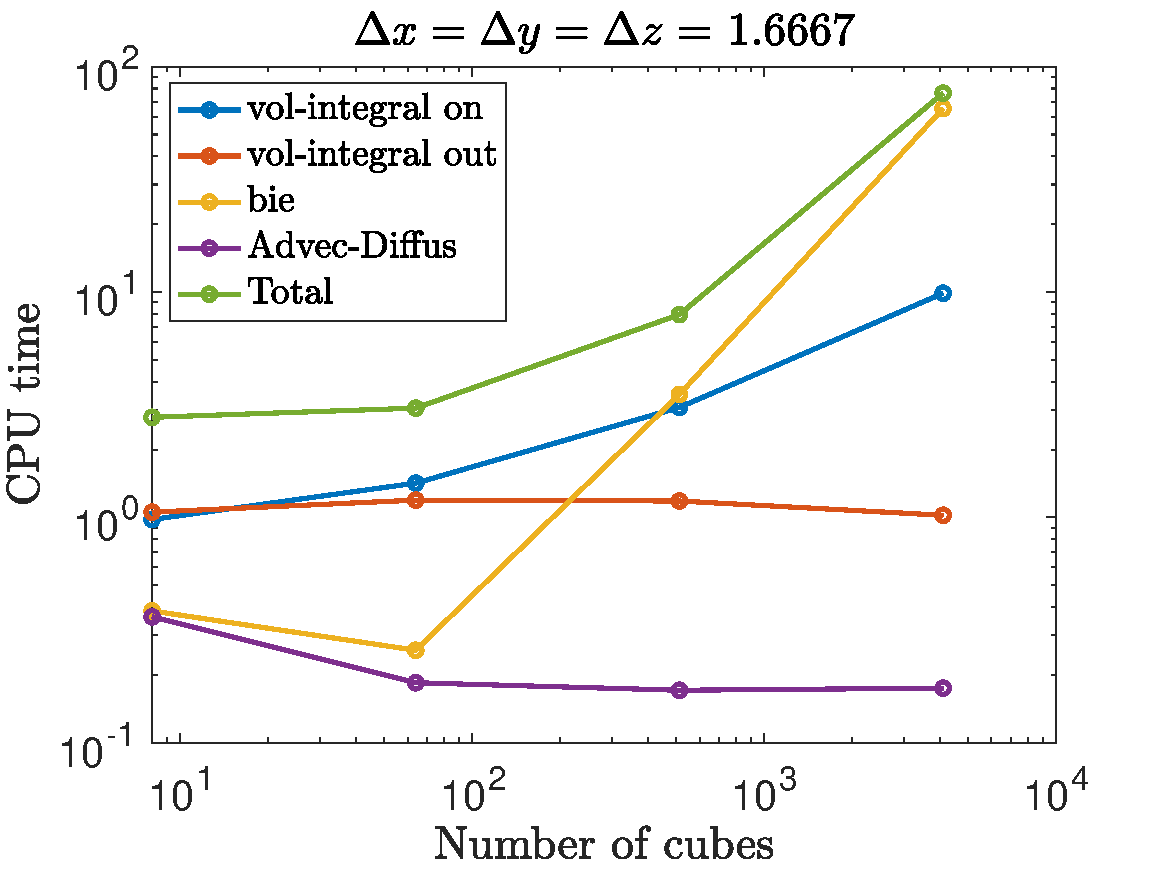
\includegraphics[scale=0.5]{./figures/fig_test_time1_fixNx}
	
	\caption{Fixed fluid domain size.}
	\label{fig_test_time1_fixNx}
\end{center}
\end{figure}

\begin{figure}[h]
	\begin{center}
		\vspace{0.5cm}
		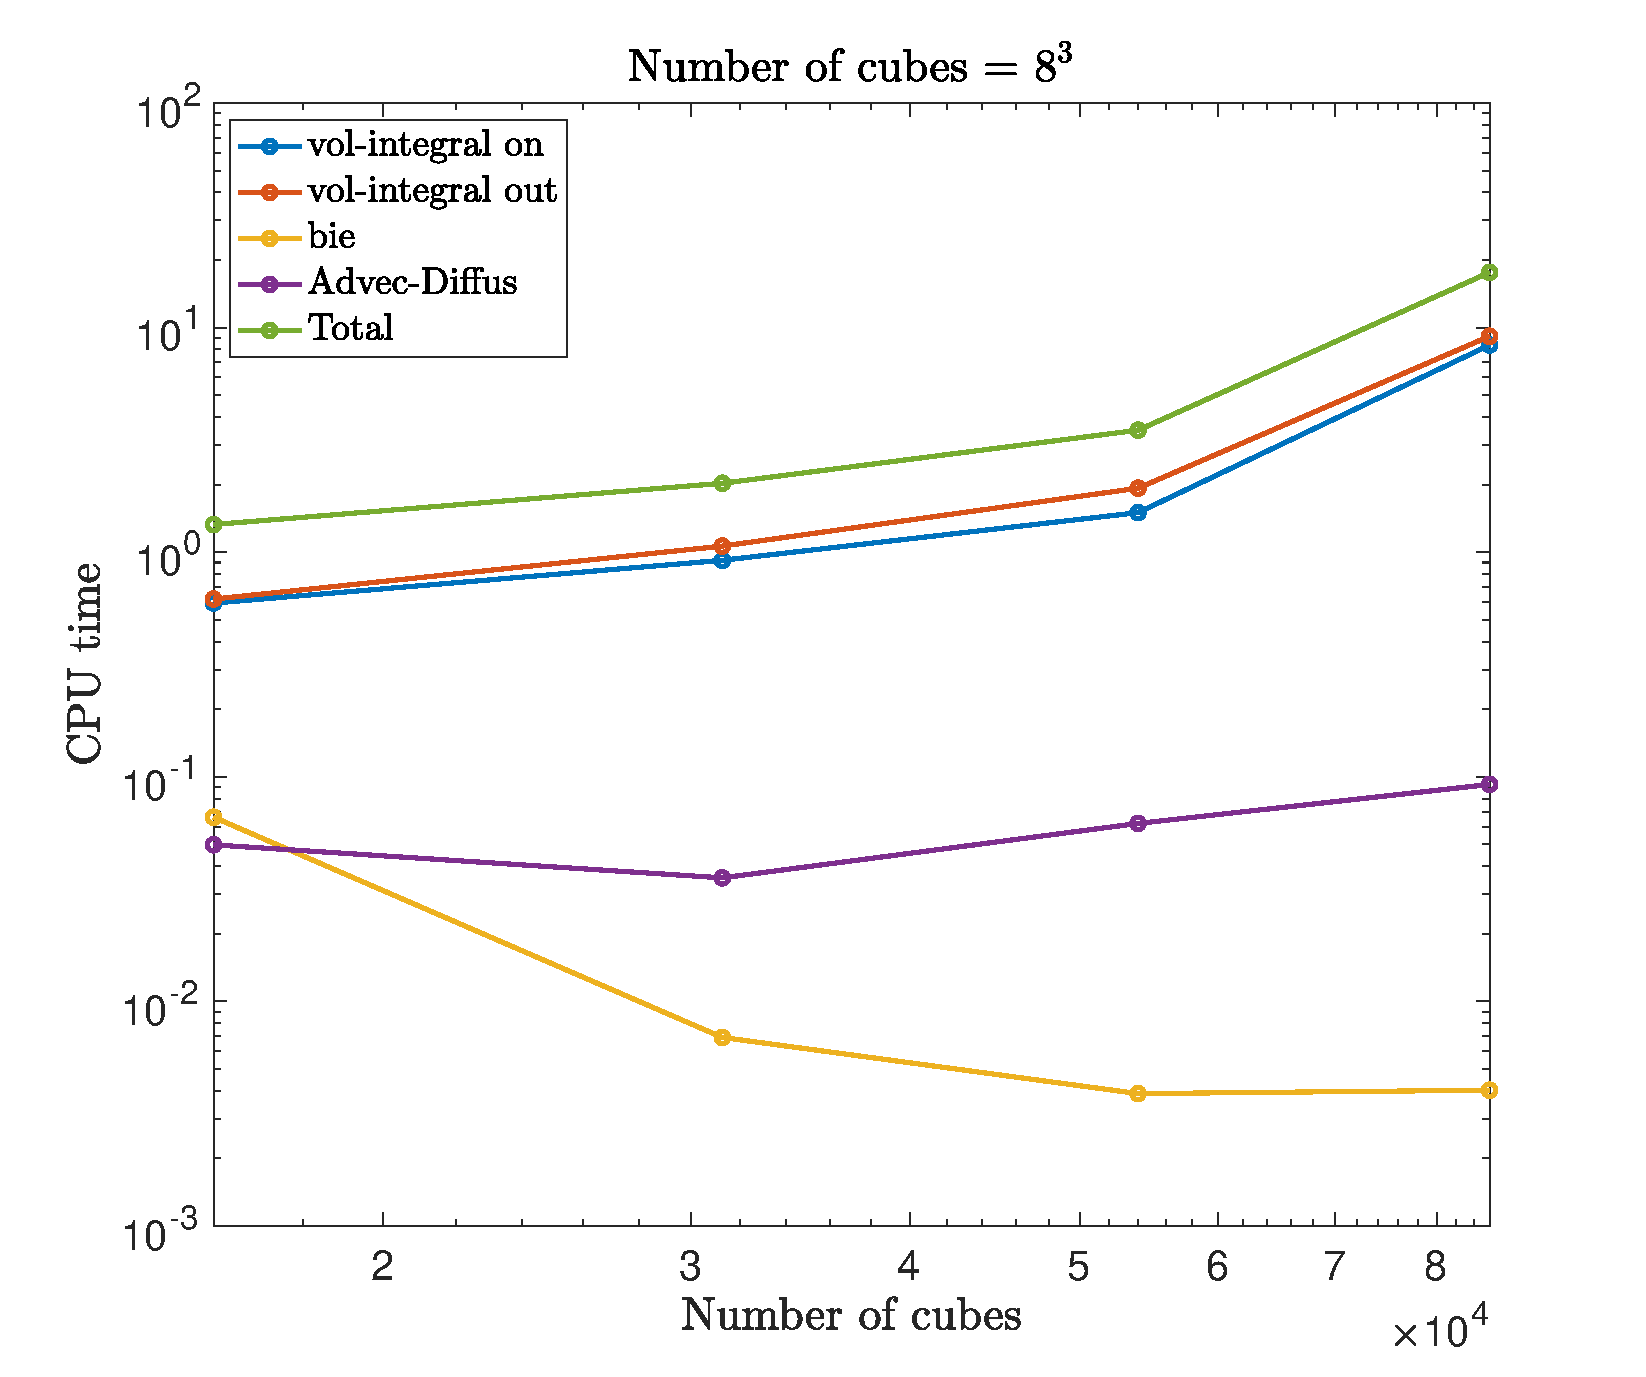
\includegraphics[scale=0.35]{./figures/fig_test_time1_varNx}
	
	\caption{Fixed aggregate size; Wrong labels. Number of cubes is $8$ and $x$-axis represents the number of total grid points. }
	\label{fig_test_time1_varNx}
\end{center}
\end{figure}

\clearpage
Today is 09/06/2022. We ran 10 time-steps for each case. The following is the setting I used to check the runtime. 
\begin{framed}
	\begin{itemize}
		\item Reference length scale: $L = 5 \times 10^{-4}$(m).
		\item Gravitational acceleration $g = 9.8$ (m$/$s$^2$).
		\item $\tilde{\mu} = 1.2 \times 10^{-3}$ (kg$/$ ms) .
		\item $\rho_s = 1.4 \times 10^{3}$ (kg$/$ m$^3$) .
		\item $\rho_0 = 1.025 \times 10^{3}$ (kg$/$ m$^3$) .
		\item $\phi = 0.9999$
		\item $\gamma = -10^{-5}$.
		\item $\alpha = 1$.
		\item $C(\vec{x}, 0) = 0$ (everywhere).
		\item Peclet number = 50.
		\\
		\item \verb+Nx = [2^3, 2^4, 2^5, 2^6]+
		\item \verb+Ny = Nx, Nz = 2Nx+
		\item Fluid domain size: $[-20, 20] \times [-20, 20] \times [-40, 40]$
		\item \verb+dt = 0.1+
		\item \verb+Nt = 10+
		\item Rotation off 
		\item \verb+NC = 8+ (Cube shape)
	\end{itemize}
\end{framed}
\begin{figure}[h]
	\begin{center}
		\vspace{0.5cm}
		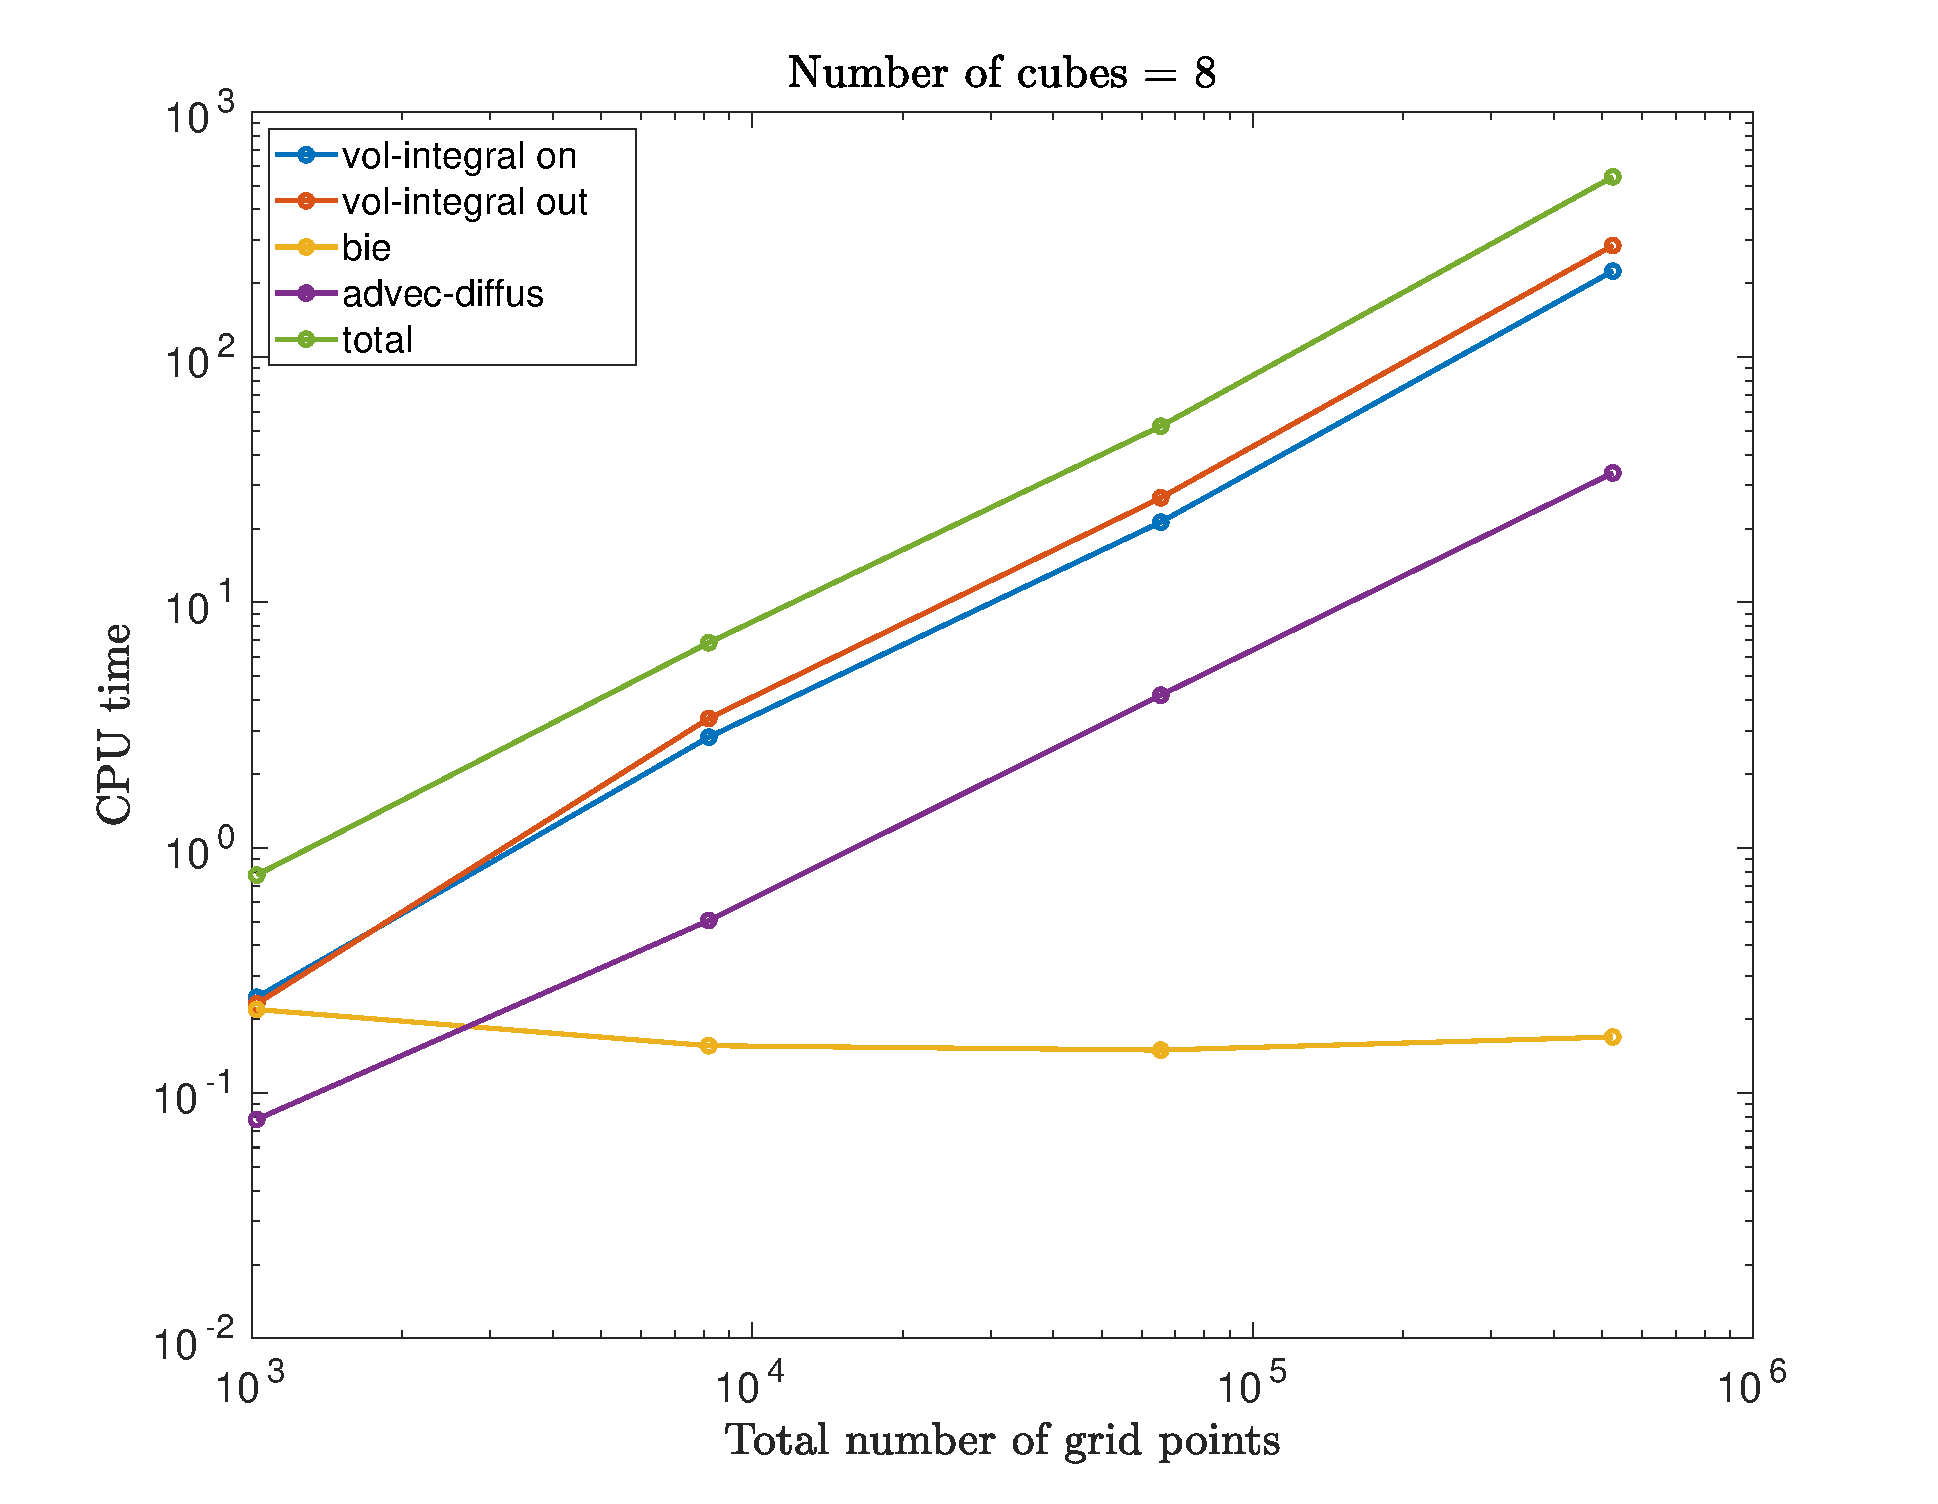
\includegraphics[scale=0.3]{./figures/fig_10time_NC8_varNx}
	
	\caption{Number of cubes is 8. }
	\label{fig_10time_NC8_varNx}
\end{center}
\end{figure}
%
% \begin{figure}[h]
% 	\begin{center}
% 		\vspace{0.5cm}
% 		\includegraphics[scale=0.33]{./figures/fig_10time_NC125_varNx}
% 		\includegraphics[scale=0.33]{./figures/fig_vel_test2-2}
	
% 	\caption{Number of cubes is 125. }
% 	\label{fig_10time_NC125_varNx}
% \end{center}
% \end{figure}
\clearpage
[Updated on 01/26/2023]
%
% \begin{figure}[h]
% 	\begin{center}
% 		\vspace{0.5cm}
% 		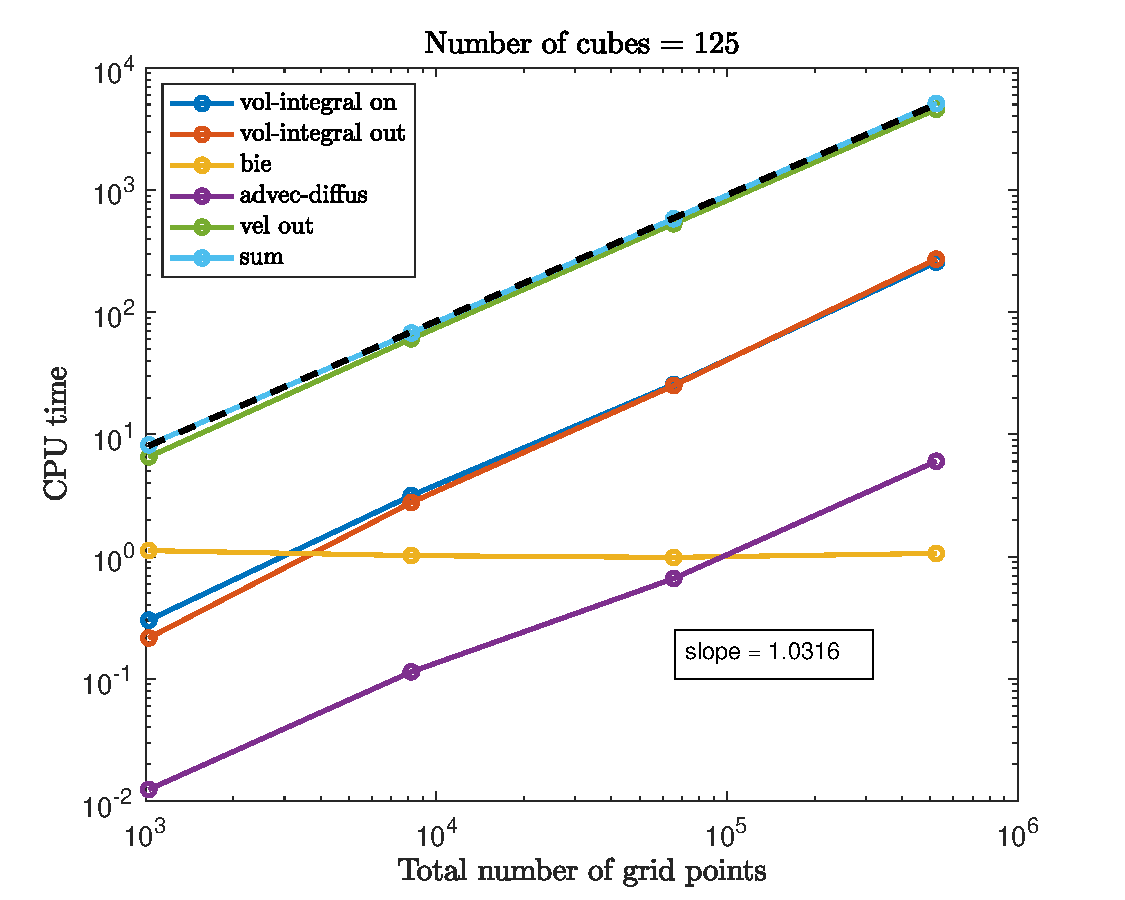
\includegraphics[scale=0.5]{./figures/fig_time_varNx5}	
% 	\caption{Number of cubes is 125.}
% 	\label{fig_time_varNx5}
% \end{center}
% \end{figure}
\begin{figure}[h]
	\begin{center}
		\vspace{0.5cm}
		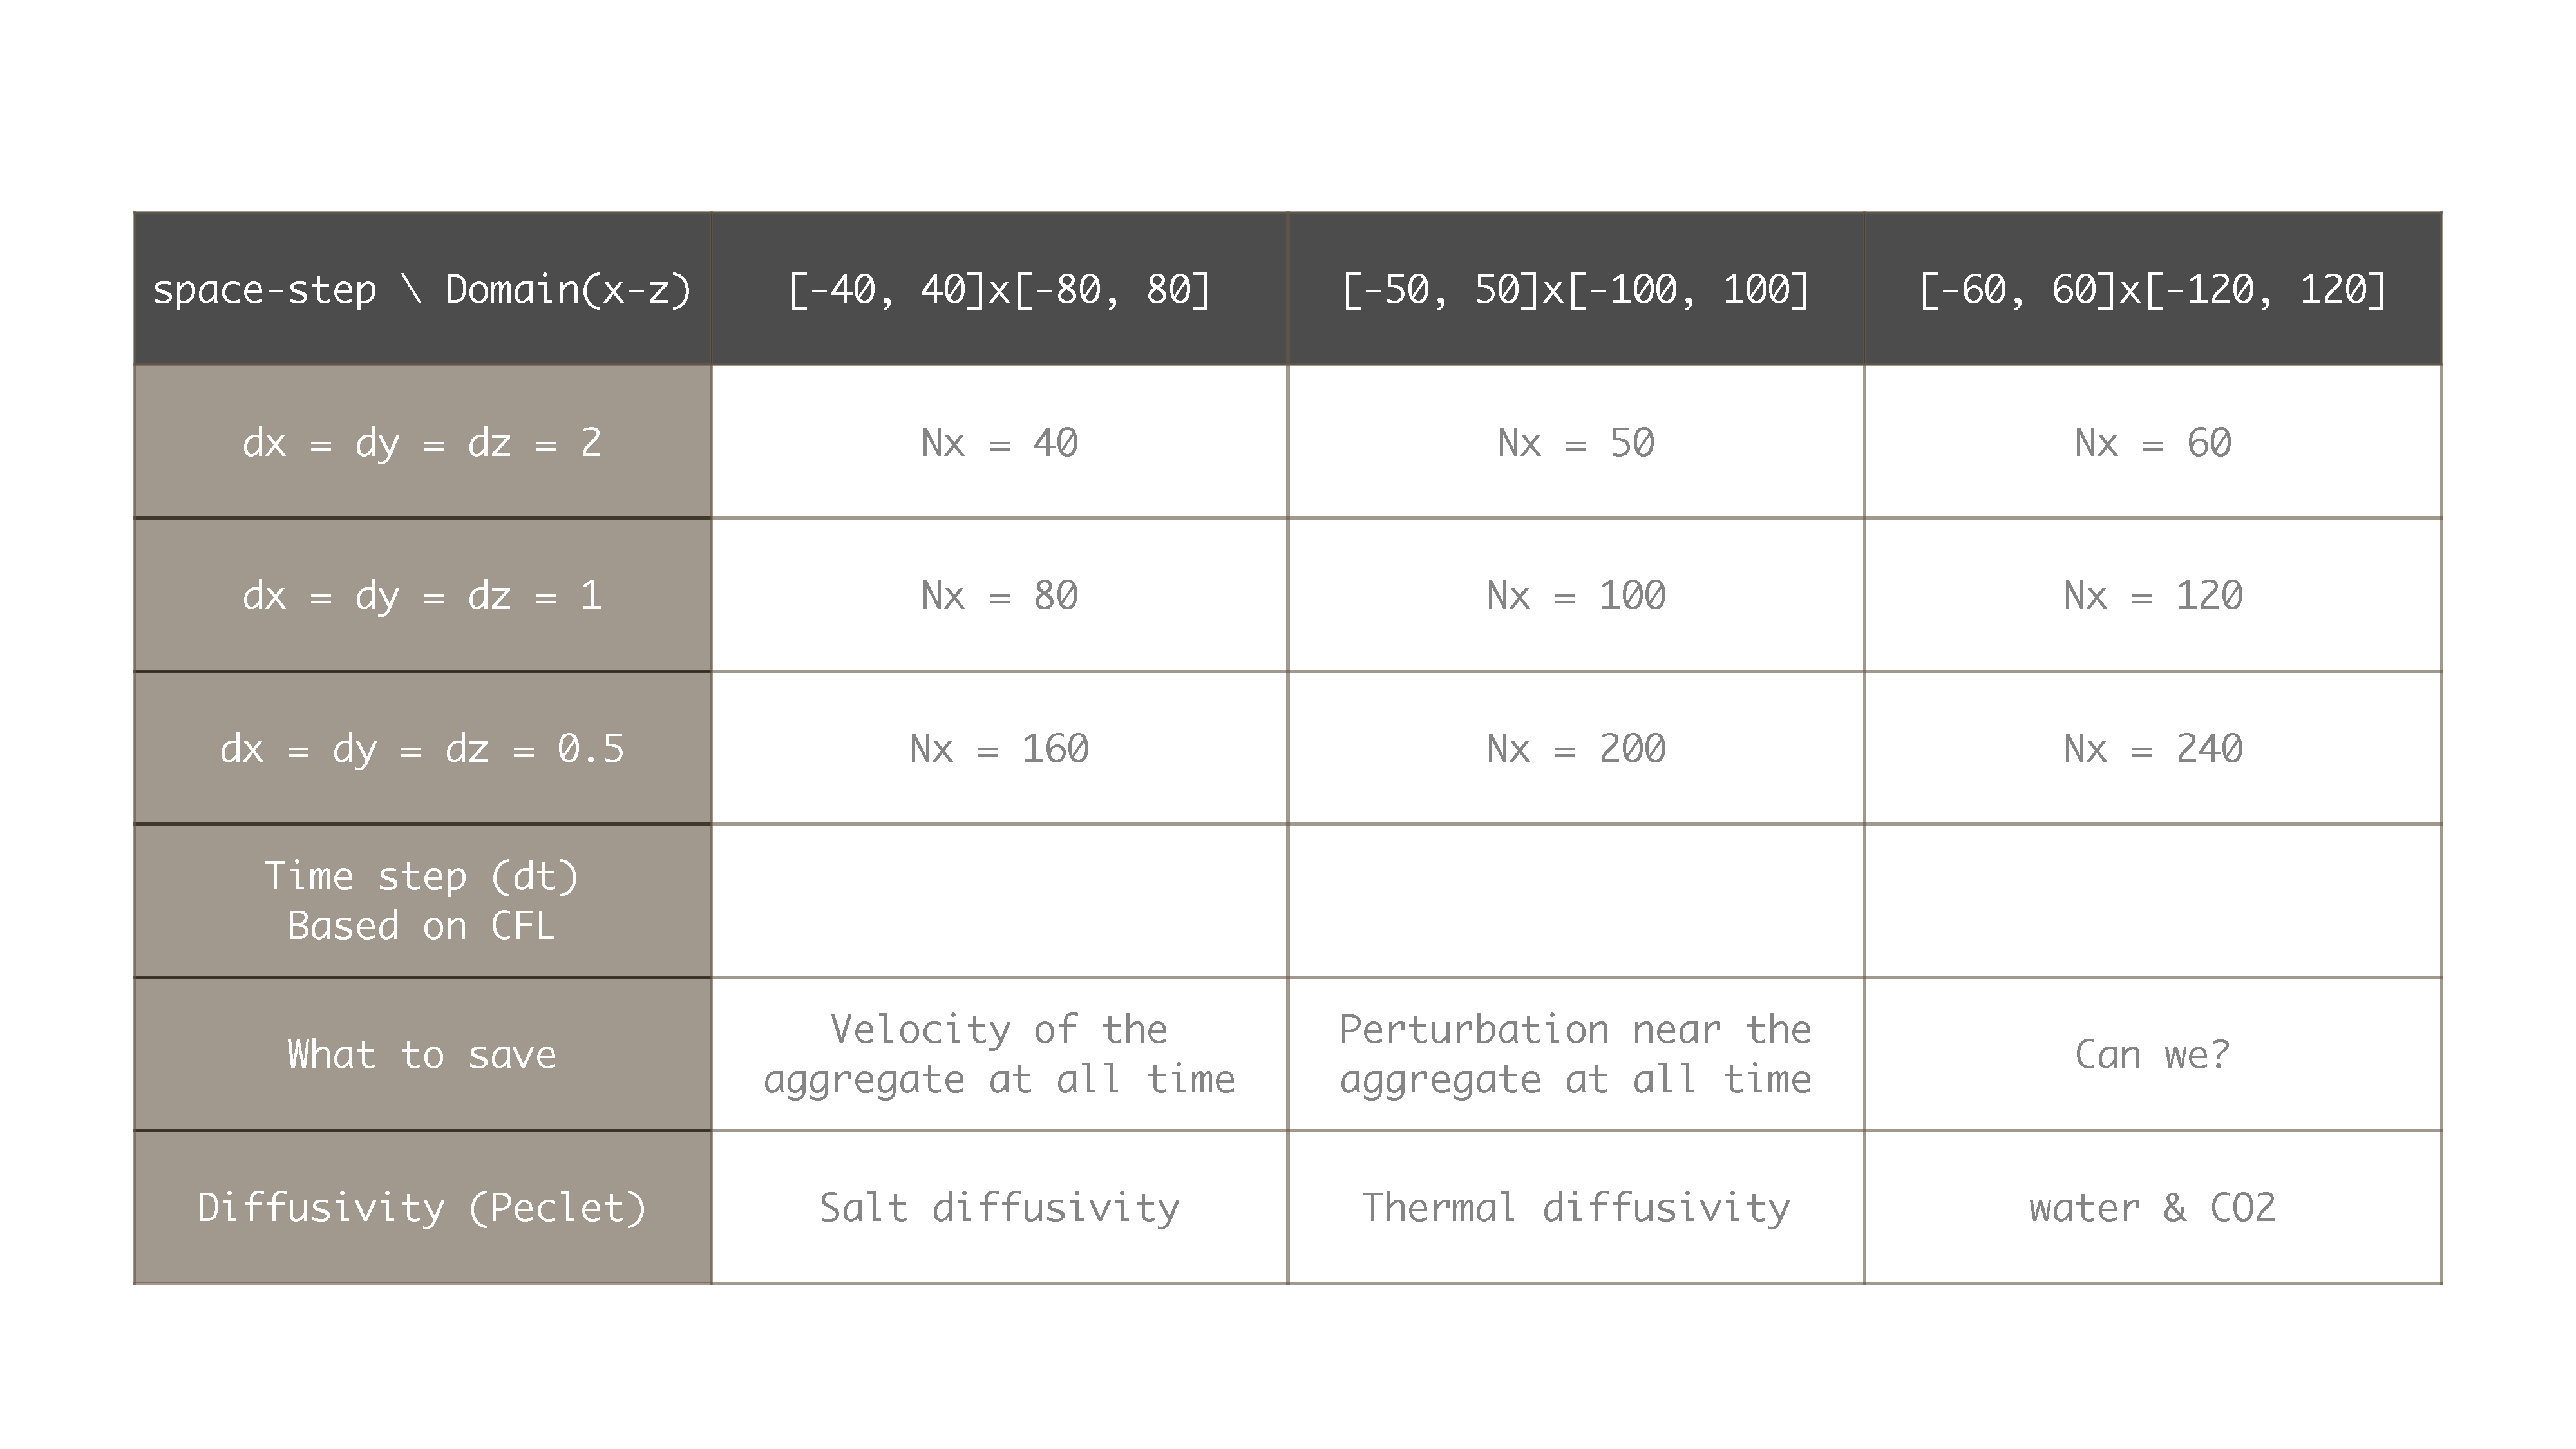
\includegraphics[scale=0.25]{./figures/table_agg_MERCED}	
	\caption{What we should run.}
	\label{fig_map_MERCED}
\end{center}
\end{figure}
\\
How can we determine the time-step size, $\Delta t$? We need to consider CFL here, for both advection and diffusion. 
\\
Knowing that the unit of diffusivity is [D] = $L^2/T$, we consider 
\[
R_{max}^2 \sim \text{Pe} \Delta t,
\]
wherer $R_{max}$ is a maximum radius of the aggregate. 
\end{comment}
\subsubsection{Homogeneous velocity}
To obtain the fluid velocity, we use the equation (\ref{eq_vel_all_onS_nonD}) for all $\vec{y} \in V$. In this computation, the homogeneous velocity part,
\begin{equation}
	u_H(\vec{y})  
	= \int_S \vec{f}(\vec{x}) \cdot \bar{\bar{G \ }}( \vec{x}, \vec{y}) \ \text{d} S(\vec{x}),
	\label{eq_uH}
\end{equation}
is quite heavy, as well as the volume integral. 
We measured CPU time while varying the total number of fluid grid points. 
In Figure \ref{fig_time_fmm_sum}, each line represents CPU time to compute (second): From the top legend 1) volume integral on the aggregate surface $S$, 2) volume integral in the fluid domain $V$, 3) solve for the linear system, 4) solve the advection-diffusion equation to update the perturbation, 5) velocity evaluation in the fluid domain, and 6) sum of all above (1 - 5).
\begin{figure}[ht]
	\begin{center}
		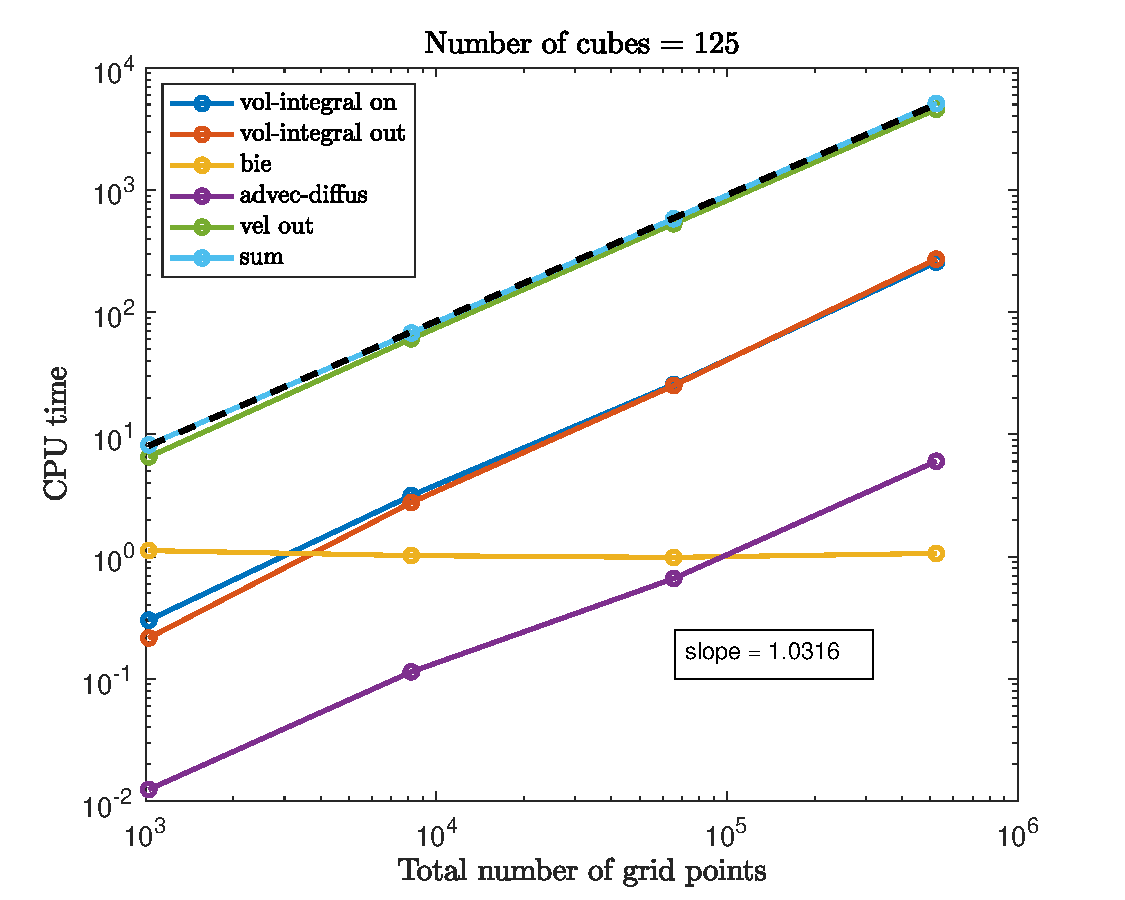
\includegraphics[scale=0.4]{./figures/fig_time_varNx5}
		% 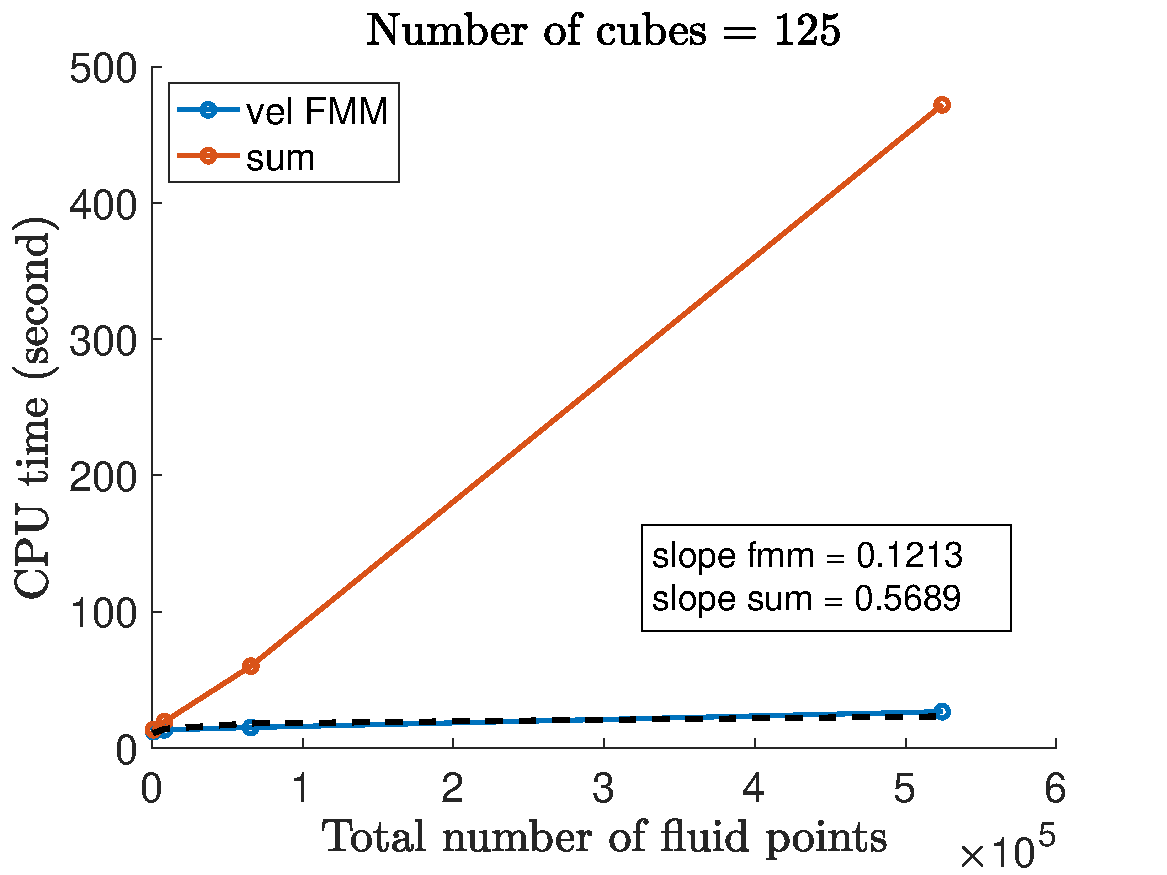
\includegraphics[scale=0.45]{./figures/fig_time_fmm_sum}
	\caption{CPU time in second with an aggregate of 125 cubes for ten time-steps.}
	\label{fig_time_fmm_sum}
\end{center}
\end{figure}
The main takeaway in this plot is that the velocity computation for all fluid points is dominant. 
We thus decided to use the FMM for this surface integral by approximating as follows:
Here, the points $\vec{x}$ is the source, and $\vec{y}$ is the target. 
For the velocity inside and on the aggregate boundary, we use the rigid boundary velocity $u(\vec{x}) = \vec{U}_a + \vec{\Omega} \times \left(\vec{x} - \vec{x}_{cm} \right)$. This implies that we do not expect any singularity in this computation ($\vec{x} \neq \vec{y}$). However, we may have a close evaluation problem. We will discuss the size of errors in the next section. We handle the integral of the Stokeslet the same as above with the volume integral. 
\par
Using the Laplace kernel, we can re-write the surface integral (\ref{eq_uH}) as
\begin{equation}
	u_H(\vec{y}) =
	\int_S 
	\vec{f}(\vec{x}) \cdot
  	\left(
  	\frac{\bar{\bar{I \ }}}{\|\vec{x} - \vec{y}\|}
  	- \left( \vec{x} - \vec{y} \right)
  	 \nabla_{\vec{y}}
  	\frac{1}{\|\vec{x} - \vec{y}\|}
  	\right)
	  \ \text{d} S(\vec{x}).
 \label{eq_surf_laplace}
\end{equation}
We first discretize the entire aggregate surface into $N_f$ number of square faces that are located at $[cx_1^n-1, cx^n_1+1] \times [cx^n_2-1, cx^n_2+1]$. This refers that $(cx^n_1, cx^n_2)$ is the center of $n-$th square face. The discretized version of the velocity equation (\ref{eq_surf_laplace}) is denoted by $H(\vec{y})$,
\begin{align}
	H(\vec{y}^m) & = u_H(\vec{y}) - E_f
	 = \sum_{n = 1}^{N_f} H^n(\vec{y}^m) 
	\nonumber \\
	& = \sum_{n = 1}^{N_f} 
	\vec{f}(\vec{x}^n) \cdot
	\int_{cx^n_2-1}^{cx^n_2+1} \int_{cx_1^n-1}^{cx_1^n+1}
  	\left(
  	\frac{\bar{\bar{I \ }}}{\|\vec{x}^n - \vec{y}^m\|}
  	- \left( \vec{x}^n - \vec{y}^m \right)
  	 \nabla_{\vec{y}^m}
  	\frac{1}{\|\vec{x}^n - \vec{y}^m\|}
  	\right)
	  \text{d} x_1  \text{d} x_2
	  ,
 \label{eq_surf_fmm_N_f}
\end{align}
% where $m = 1, \  2, \cdots, \ M$, and $M$ is the total number of targets (where we want to obtain the velocity). 
 Note that the stress $\vec{f}(\vec{x}^n)$ is assumed to be constant over each square face. The error coming from this approximation is denoted as $E_f$; its error analysis is discussed in our previous paper \cite{yoo_hydrodynamic_2020}. One can find that we have the largest error at the cube's corner. We would like to keep this true as we make further approximations. 

\par
Next, we need to approximate the surface integral in equation (\ref{eq_surf_fmm_N_f}) using a Riemann sum,
\begin{align}
	\tilde{H}^n(\vec{y}^m) 
	& = H^n(\vec{y}^m) - E_{G} 
	\nonumber \\ 
	& =
	\sum_{n = 1}^{N_f} 
	\vec{f}(\vec{x}^n) \cdot
	\sum_{s=1}^{Ns^2} d^2 
  	\left(
  	\frac{\bar{\bar{I \ }}}{\|\vec{x}_s^n - \vec{y}_s^m\|}
  	- \left( \vec{x}_s^n - \vec{y}^m \right)
  	 \nabla_{\vec{x}_s^n}
  	\frac{1}{\|\vec{x}_s^n - \vec{y}^m\|}
  	\right)
	  + E_{G},
 \label{eq_surf_fmm_N_f_n}
\end{align}
where $E_G$ is the error coming from the quadrature method. 
We make $Ns$ number of sub-squares that have sizes of $d = 2/Ns$, and take the center of each sub-squares as the integration points. 
We take the same number of points, $Ns$, evenly distributed in one direction. We can also consider the number of points as the number of sub-squares in one face. 
In the following schematics, Figure \ref{fig_face_grid}, the red cross represents the center of the $n-$th square face, $(cx^n_1, cx^n_2)$.
\begin{figure}[h]
	\begin{center}
		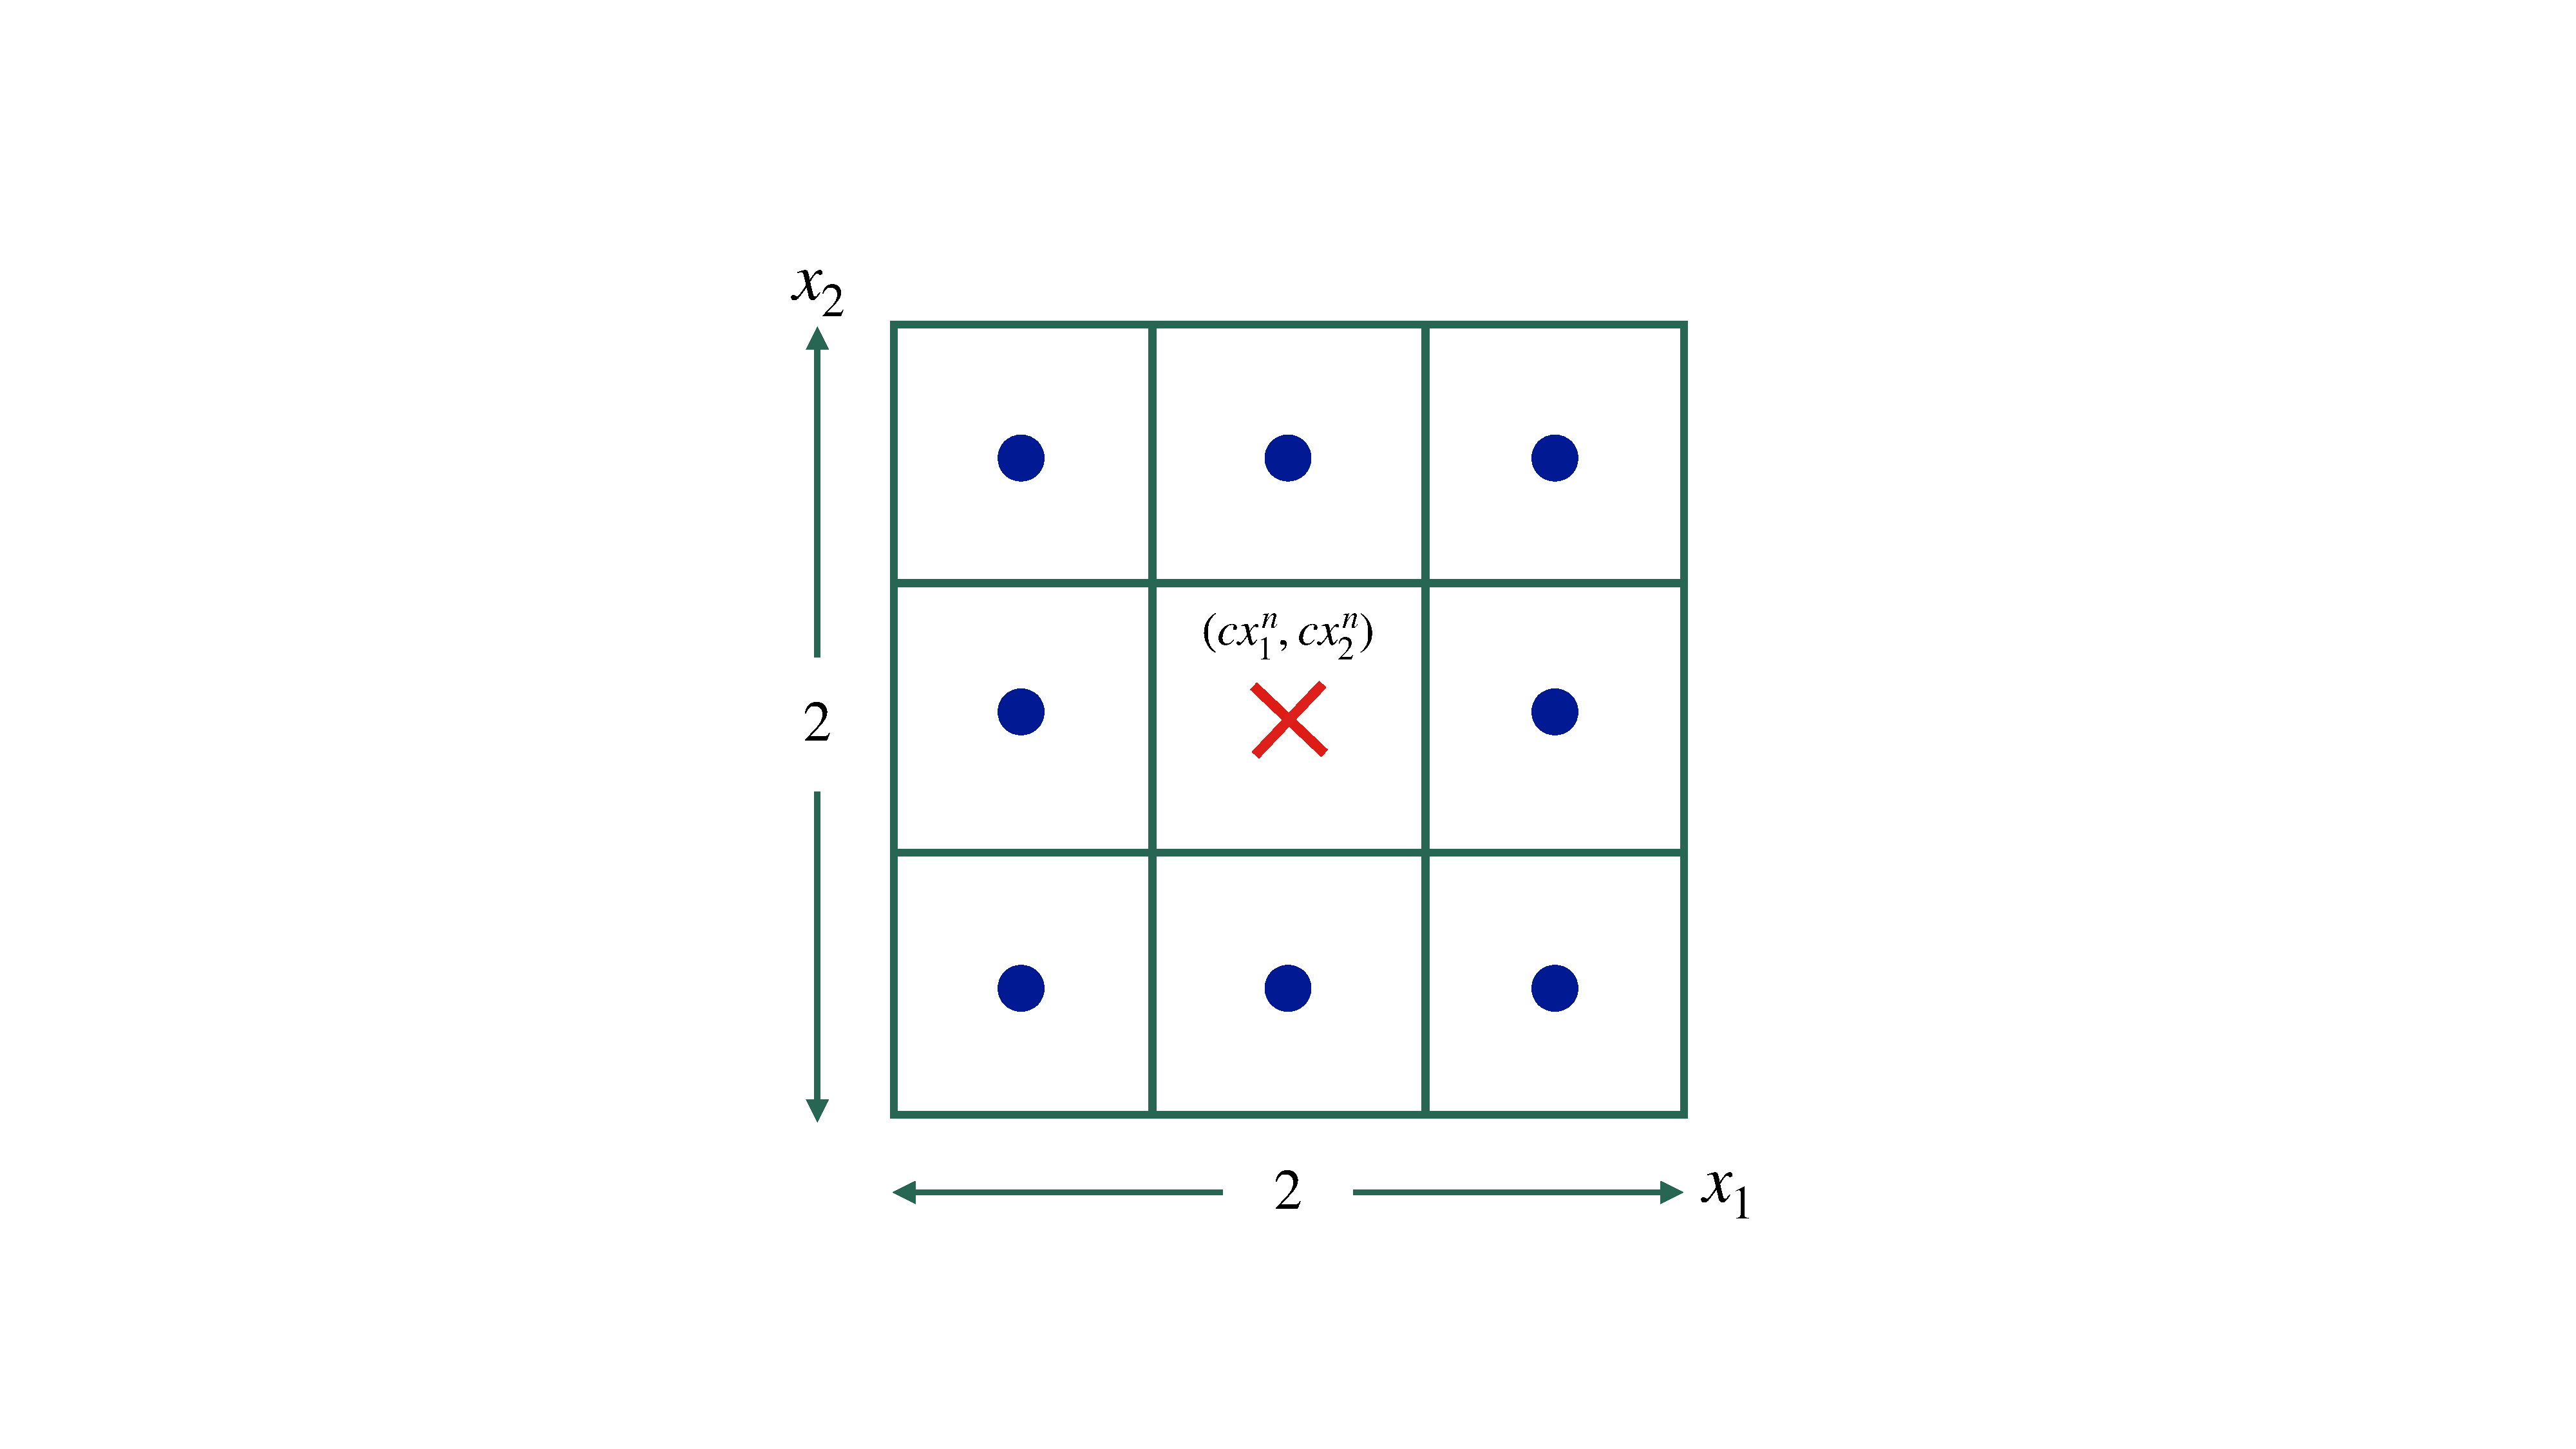
\includegraphics[scale=0.17]{./figures/fig_face_grid}
	\caption{Schematic of points we use to approximate the integral of the single-layer potential kernel over one square face.}
	\label{fig_face_grid}
\end{center}
\end{figure}
Including the center (the red cross in Figure \ref{fig_face_grid}), the blue dots are the integration points.
We may not include any boundary values on one square face for simplicity.
\par
As mentioned, we hope to have a reasonable size of the integration error, i.e., $E_G \ll E_f$.
To measure $E_f$, we consider the settling of one cube shape aggregate.
We then observe the relative error of the vertical velocity on one square face, considering the translational velocity, $\vec{U}_a$, as the exact solution.
\begin{figure}[h]
	\begin{center}
		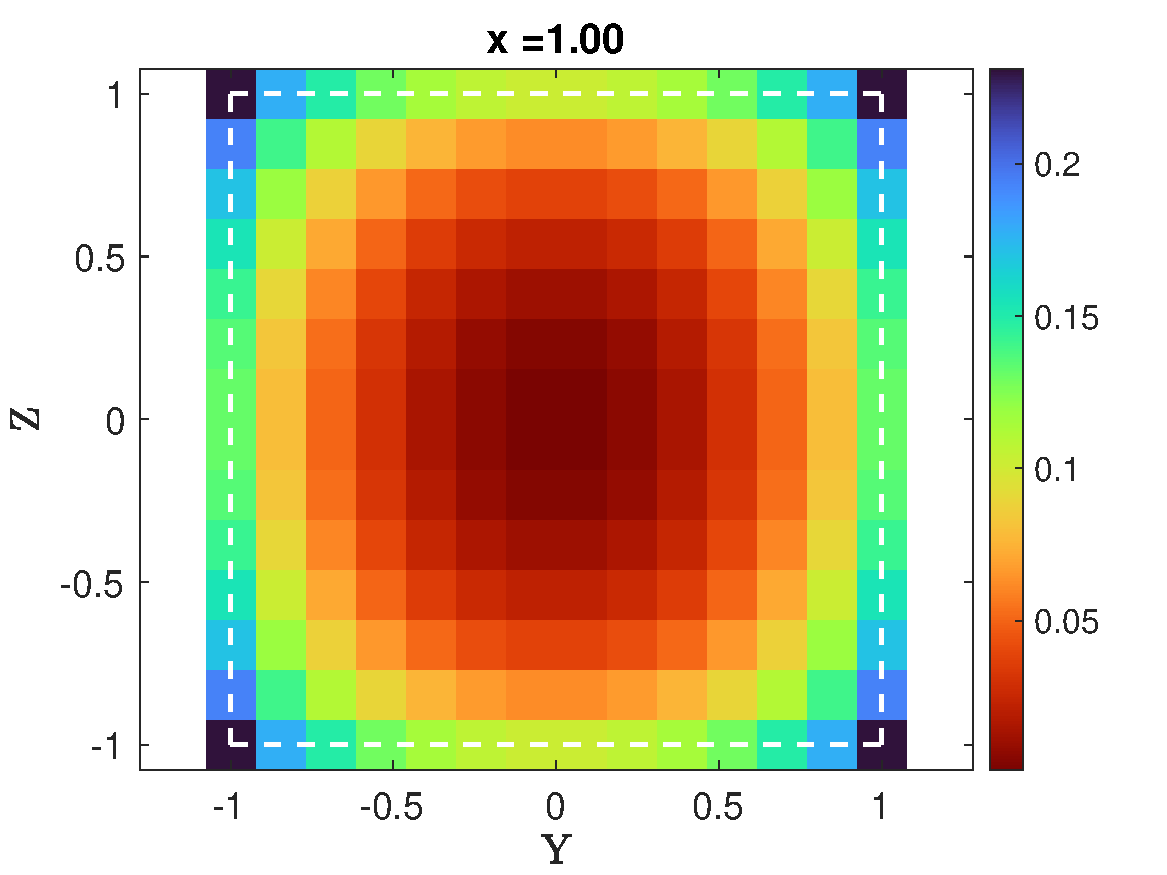
\includegraphics[scale=0.3]{./figures/fig_corner_err}`'
	\caption{Relative error of }
	\label{fig_corner_err}
\end{center}
\end{figure}
In Figure \ref{fig_corner_err}, we see the square face at $x = 1.00$, where the white dashed line shows the location of the square face, and the color indicates the relative error. It implies that the maximum of 23.12$\%$ error occurs at the cube's corner, as we expected. We thus would like to regulate the quadrature error, $E_G$, by adjusting the total number of integration points, $Ns^2$.
\par
Specifically, we explain two types of errors by letting $u_H(\vec{y})  = U = F \cdot  G$ be the exact or true velocity. Then 
\begin{align}
	U^* = F^* \cdot  G
	\\
	U^{*+} = F^* \cdot  G^+
\end{align}
where $F = F^* + E_f$ and $G =  G^+ + E_G$.
By approximating the integral of the kernal, using FMM3D, we compute $U^{*+}$, that is,
\begin{align}
	U^{*+} = (F-E_f) \cdot (G - E_G) 
	% \nonumber \\
	% = F \cdot G - F \cdot E_G - G \cdot E_f 
	% + E_f \cdot E_G
	% \\
	= U +  \left| E_f \cdot G + F  \cdot E_G \right|  + \mathcal{O}(E_f E_G).
\end{align}
We know that 
\[
	|U-U^*| = |E_f \cdot G| \approx 23 \%,
	\]
and we would like to have
\[
	|F  \cdot E_G| \ll	|E_f \cdot G |
\]
Note that 
\[
	  |F \cdot E_G| = |F^* \cdot E_G + E_f \cdot E_G|
	  \approx |F^* \cdot E_G |
\]
Thus, what we need to compare is two velocity approximations,
\begin{align}
	|U^* - U^{*+}| =| F^* \cdot E_G| \ll 23 \%
	\label{eq_condition_EG}
\end{align}

Following the above analysis, there are two parameters we can choose for efficiency: 1) the number of quadrature points and 2) the tolerance $\varepsilon$ in the FMM3D library. 
When we use the FMM3D library, we can choose the desired accuracy, $\varepsilon$, which determines the number of terms in the series expansion. We want to select an appropriate $\varepsilon$ since small ones increase the computation time. 
In Figure \ref{fig_Ef_EG_compare}, we vary the number of integration points to choose an optimal value. 
\begin{figure}[ht]
	\begin{center}
		% 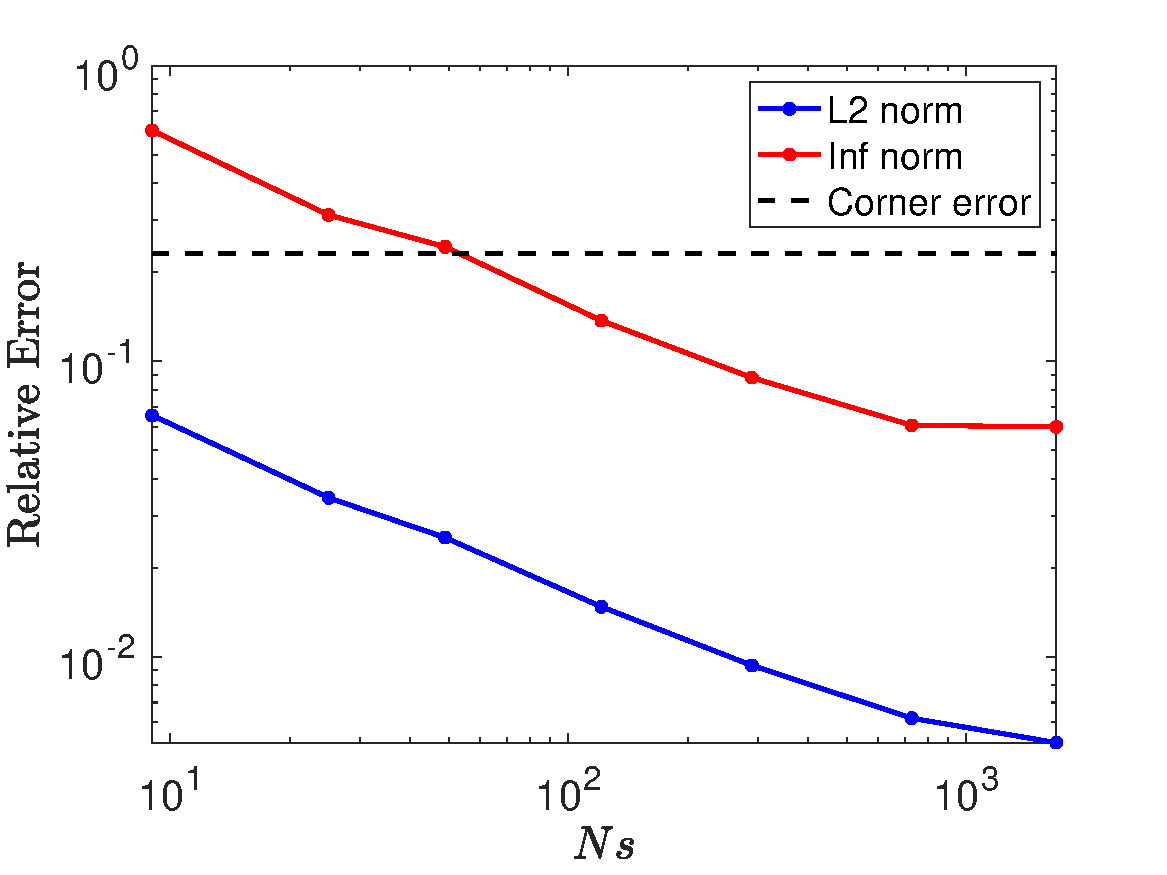
\includegraphics[scale=0.33]{./figures/fig_Ef_EG_compare}
		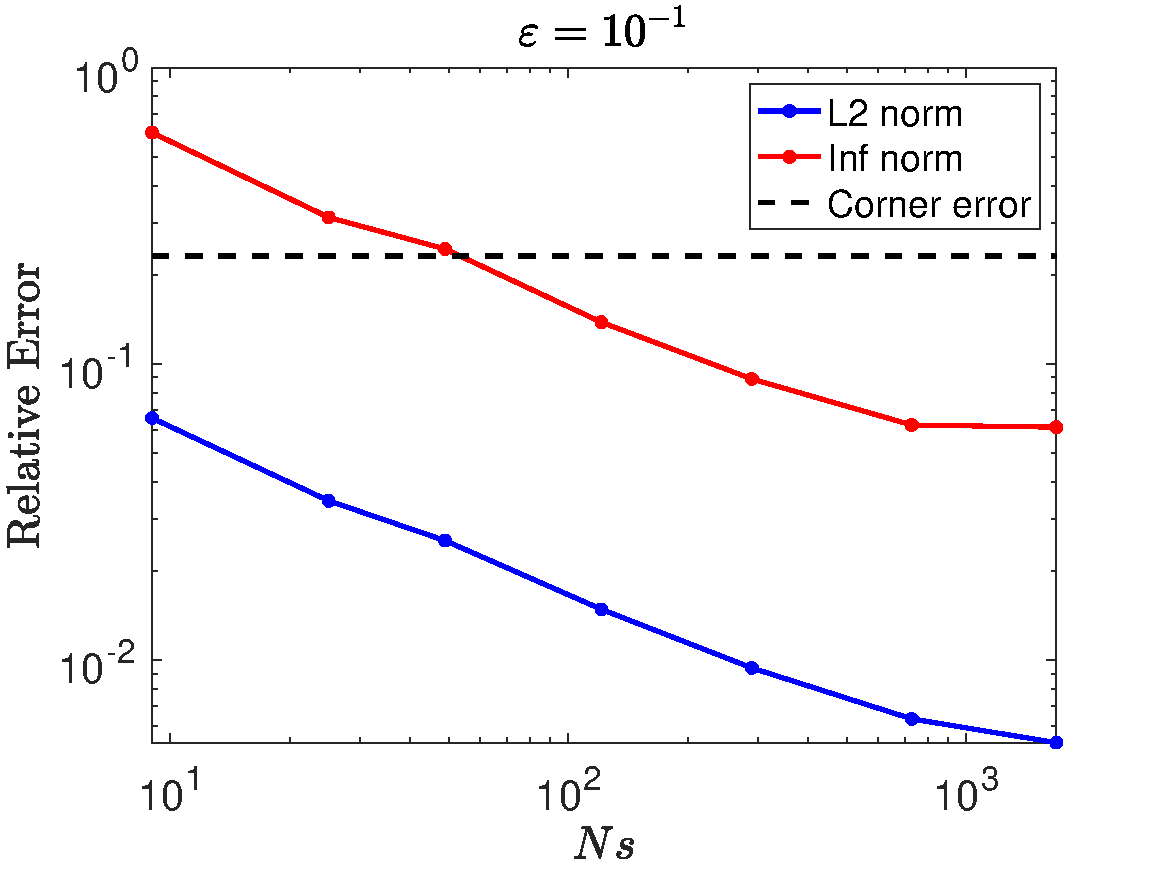
\includegraphics[scale=0.4]{./figures/fig_Ef_Eg_ep-1}
	\caption{Relative error between $U^*$ and $U^{*+}$, varying the number of integration points: $Ns = [3, 5, 7, 11, 17, 27,41]^2$ and $\varepsilon = 10^{-1}$.}
	\label{fig_Ef_EG_compare}
\end{center}
\end{figure}
We test a single-time simulation in the domain,  $[-5, 5] \times [-5, 5] \times [-10, 10]$,  with one cube aggregate model. To confirm the responses of $\varepsilon$ values, we simulate the same one with two tolerance values, $\varepsilon = 10^{-1}, \ 10^{-6}$.
From this analysis, we are convinced that $Ns = 9^2$ quadrature points are enough to satisfy what we want in equation (\ref{eq_condition_EG}). It produces quite similar results for the $\varepsilon = 10^{-6}$ case. We did not notice any difference in accuracy. We may observe this because the corner error, $E_f$, dominates our approximation and is already larger than $10 \%$. 

After we implemented the FMM3D library into our program, we timed one more time to compare the fluid velocity computation shown as the green (or dashed line) in Figure \ref{fig_time_fmm_sum}. It is clear that the efficiency of the computation increases about ten times. 
\begin{figure}[ht]
	\begin{center}
		% 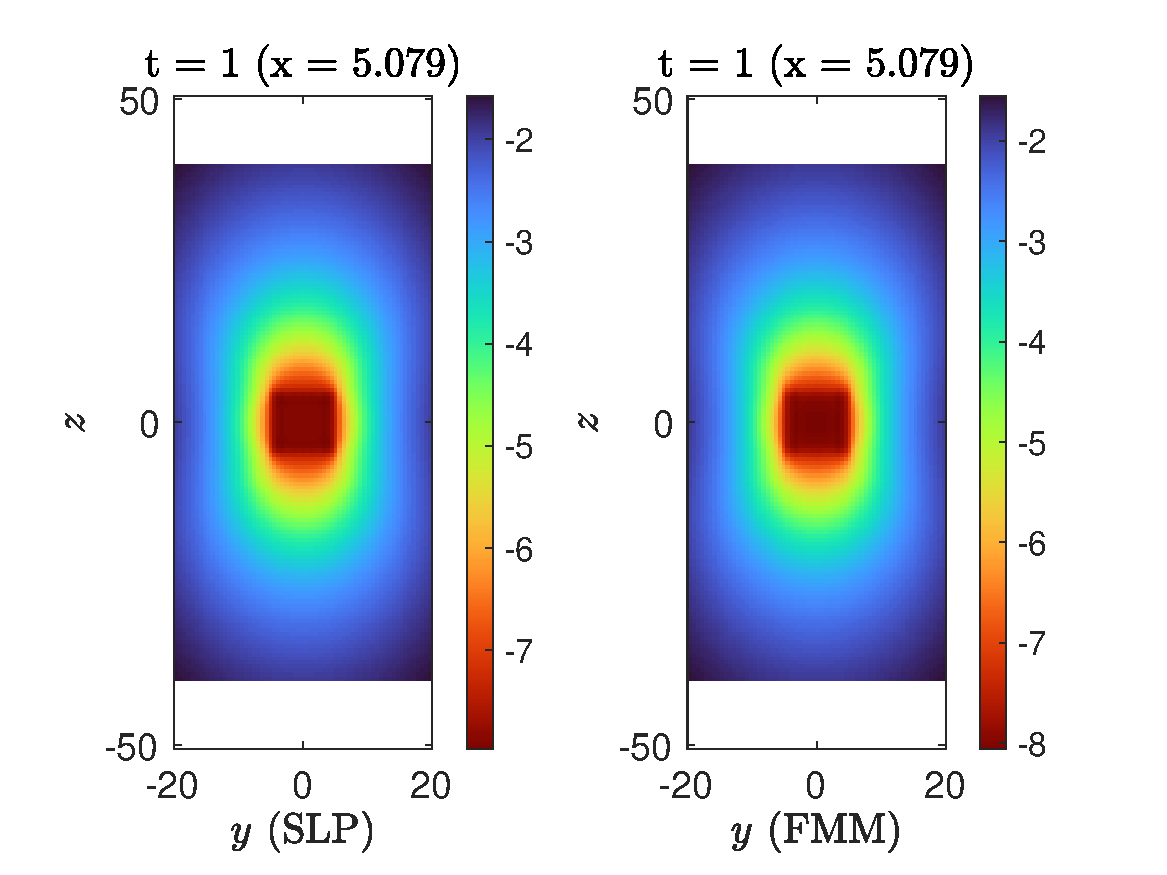
\includegraphics[scale=0.42]{./figures/fig_vel_mm5_t1}
		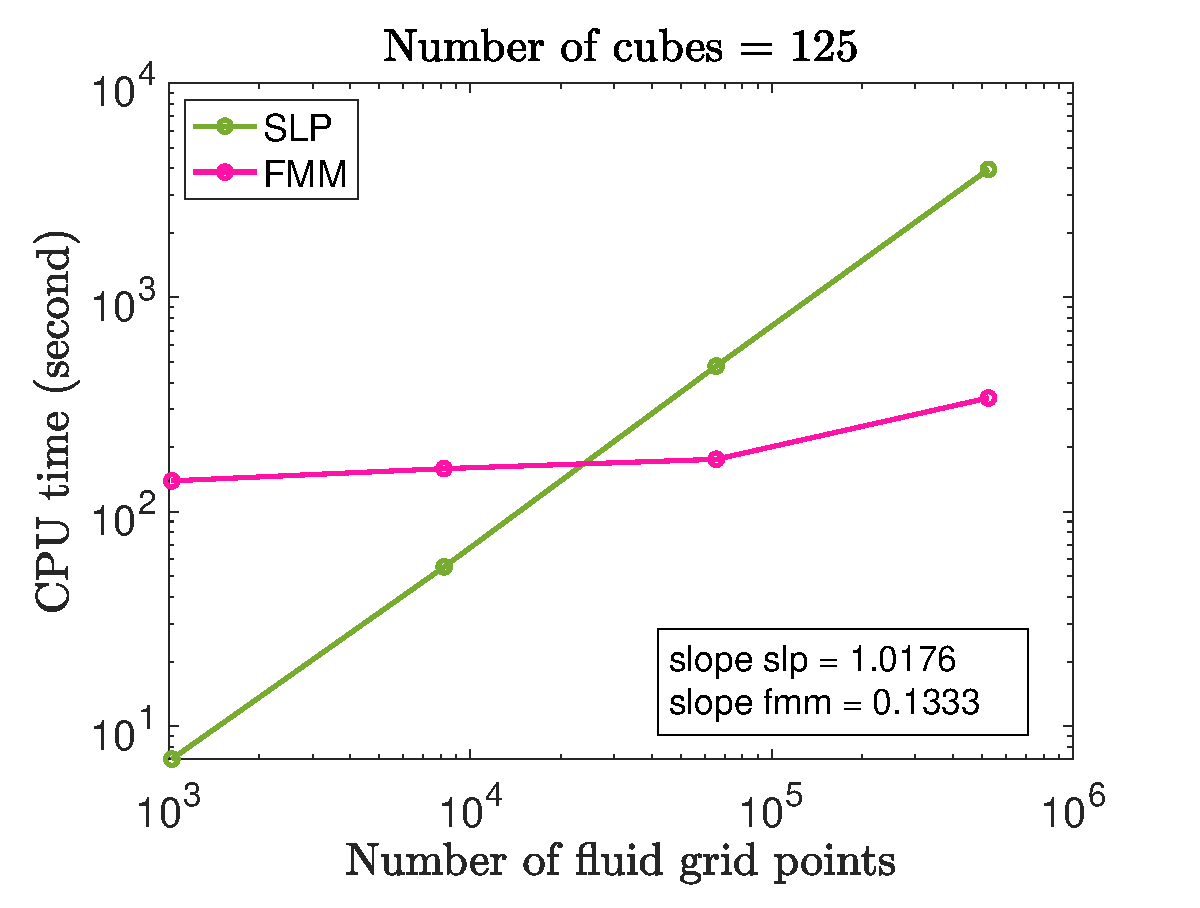
\includegraphics[scale=0.4]{./figures/fig_time_both_mm5_Nt10}
	\caption{CPU time with an aggregate made with 125 cubes for tem time steps. The blue line is the original homogeneous solution, and the orange represents the approximation using the FMM3D library.}
	\label{fig_vel_mm5_t1}
\end{center}
\end{figure}

% \clearpage
% On January 27, 2023, we decided to check in the timing and memory capacity to use the Pinnacles. I am going to test both SLP and FMM versions, separately, just to make sure if FMM is converging to the correct velocities. Here are the paratmesters we are going to use for this experiment:
% \begin{framed}
% 	\begin{itemize}
% 	\item \verb+NC = [50, 100]+ (Random shape {\color{red}$\rightarrow$ check the Nf}) 
% 	\item \verb+Nx = [60, 120]+
% 	\item \verb+Ny = Nx, Nz = 2Nx+
% 	\item Fluid domain size: Make $\Delta x =\Delta y = \Delta z = 1$.
% 	\item $\Delta t = 0.5$
% 	\item \verb+Nt = 100+ (Final time would be 50.)
% 	\item Pe = 0.5 ( = $\Delta t$)
% 	\item {\color{blue} Save at 1) the final time only AND 2) every time step: velocity, C, $U_a$ with location, $\Omega$, $\theta$ (rotaion angle)}
% 	\end{itemize}
% \end{framed}



% \begin{figure}[h]
% 	\begin{center}
% 		\vspace{0.5cm}
% 		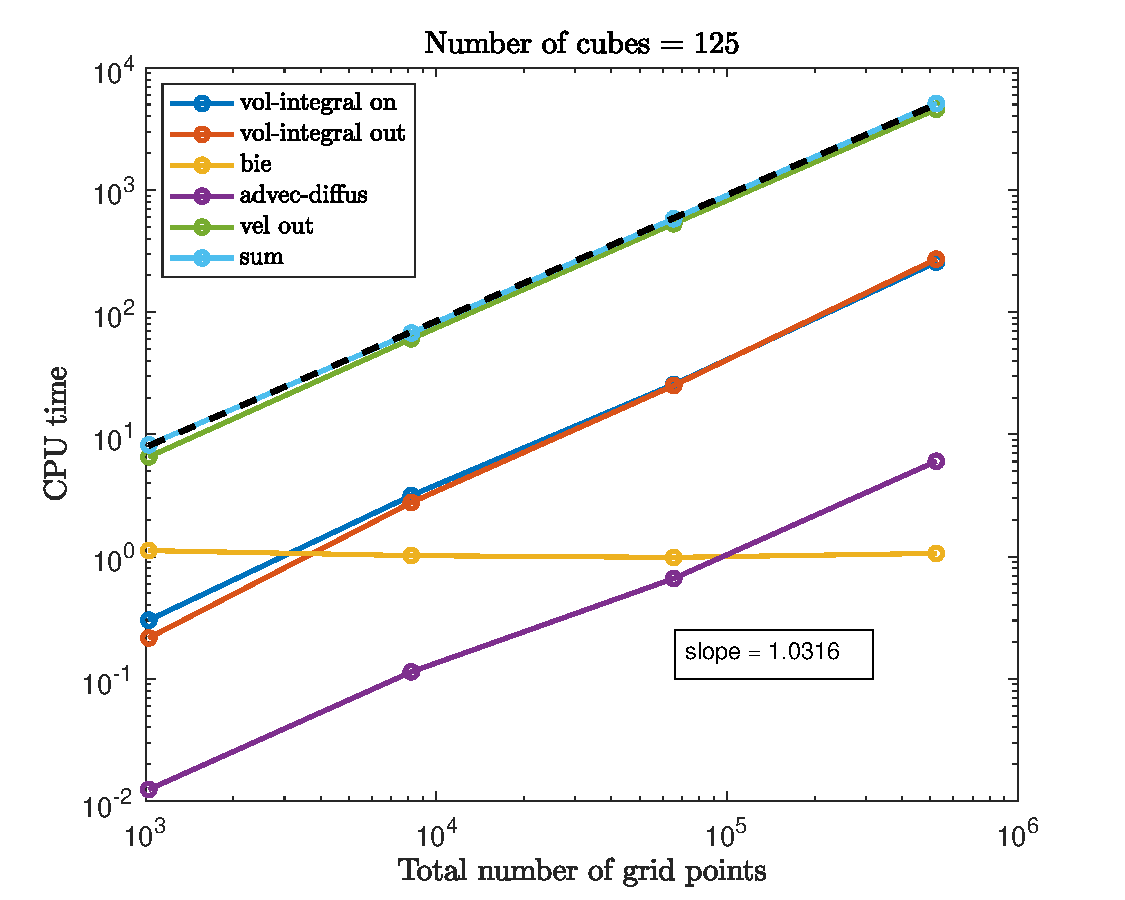
\includegraphics[scale=0.5]{./figures/fig_time_varNx5}	
% 	\caption{Number of cubes is 125.}
% 	\label{fig_time_varNx5}
% \end{center}
% \end{figure}
\begin{comment}
\clearpage
\begin{itemize}
	\item How did you code up exactly to use FMM3D?
	\item you may introduce index notations for this"  $i,j = 1,2,3$ works twice = 18 times  
	\item What is the main difference between volume integral and this surface integral?
	\item {\color{red} We expect to use total 18 times of FMM3D library to compute the entire velocity field.$\rightarrow$ why?}
\end{itemize}
In order to validate the code, measure the error size, and check the computation time, we consider a homogeneous case.
Error plots - compare the $U_a = -0.3470$ values.
\begin{figure}[h]
	\begin{center}
		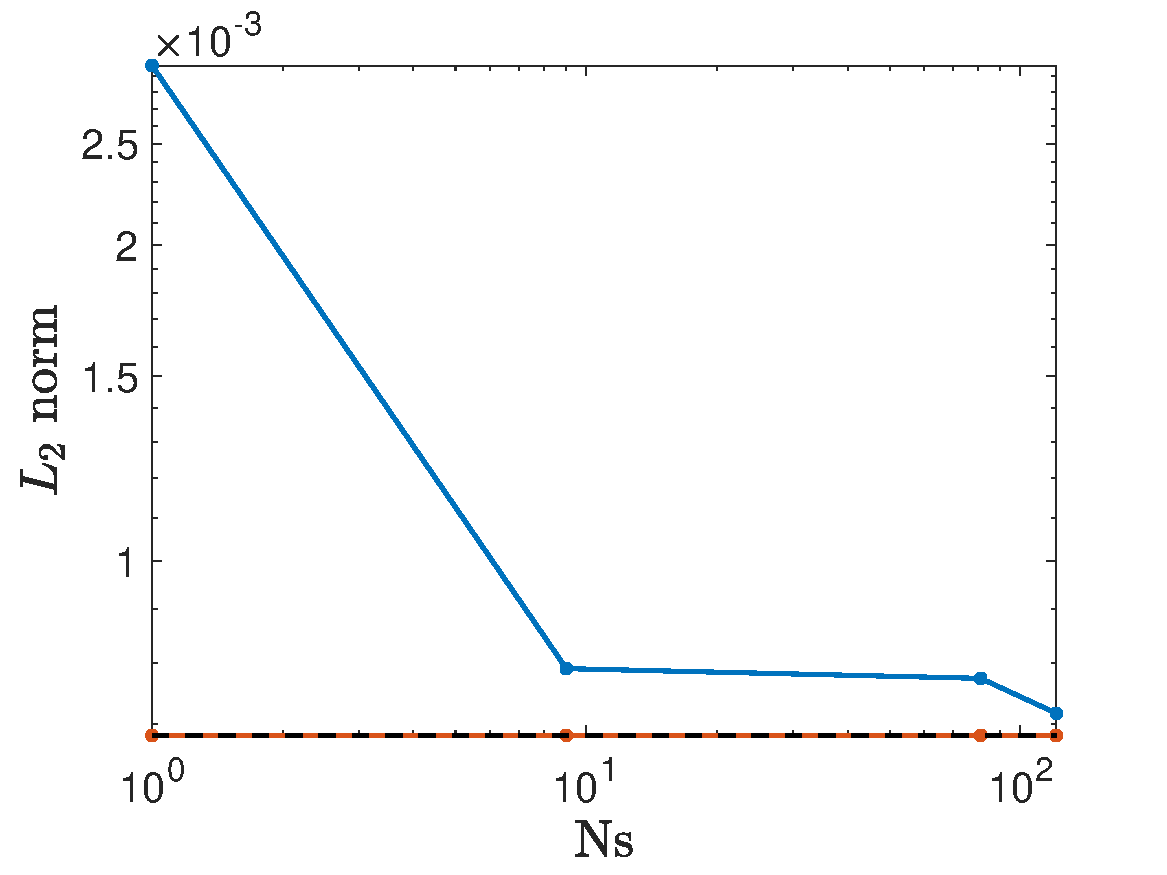
\includegraphics[scale=0.4]{./figures/fig_cornerErr_L2}
		\includegraphics[scale=0.4]{./figures/fig_cornerErr_iN_f}
	\caption{(Left) Velocity plot of one face. 1 point is used to approximate the surface integral of $G$ kernel using FMM. (Right) $11^2$ point is used to approximate the surface integral of $G$ kernel using FMM. }
	\label{fig_cornerErr}
\end{center}
\end{figure}
\end{comment}
%Rotation---------------------------------------------------
\clearpage
\section{Validation}

\section{Simultation results}
To somewhat justify our tiny stability issue, we compare the results between two different time step sizes: $\Delta t = 0.25 , \ 0.5$.
\begin{figure}[ht]
	\begin{center}
		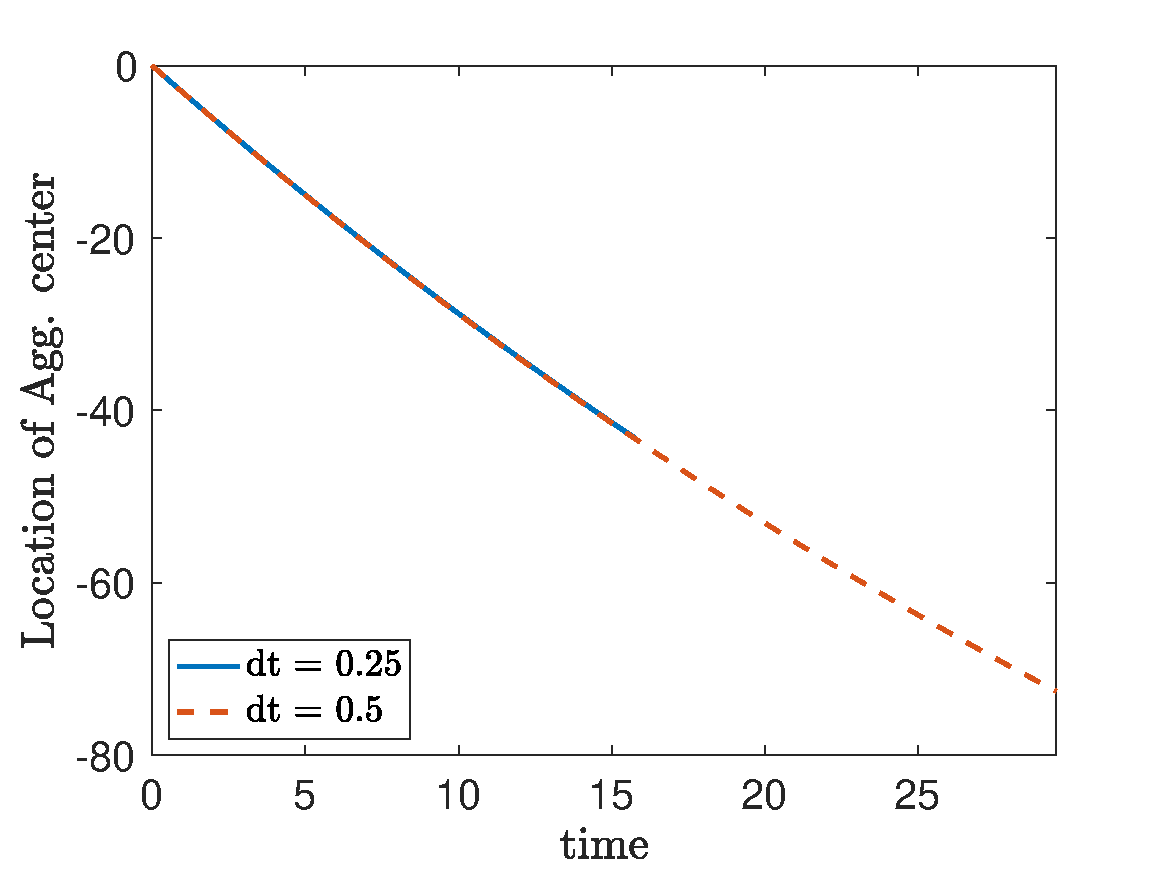
\includegraphics[scale=0.33]{./figures/fig_NC50_compare_dt_cm3_all}
		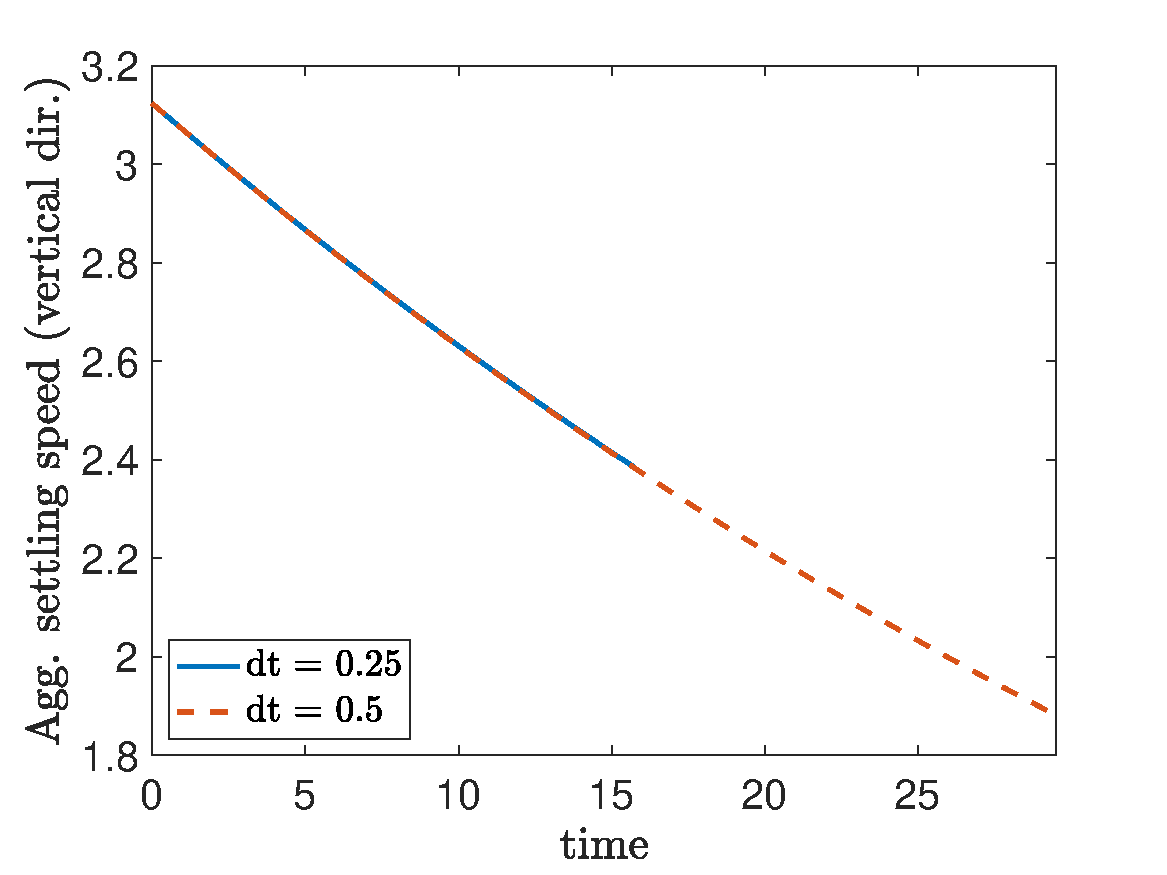
\includegraphics[scale=0.33]{./figures/fig_NC50_compare_dt_Ua3_all}
		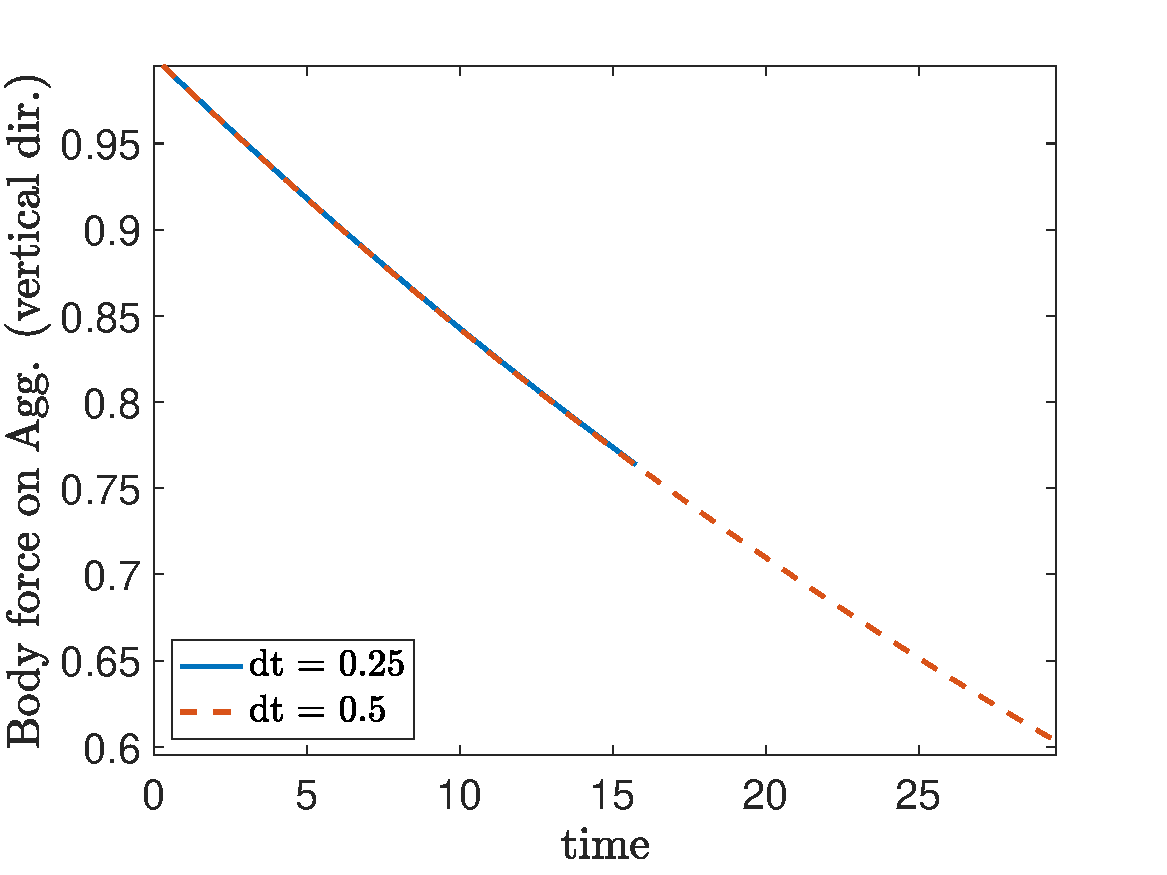
\includegraphics[scale=0.33]{./figures/fig_NC50_compare_dt_Fo3_all}
		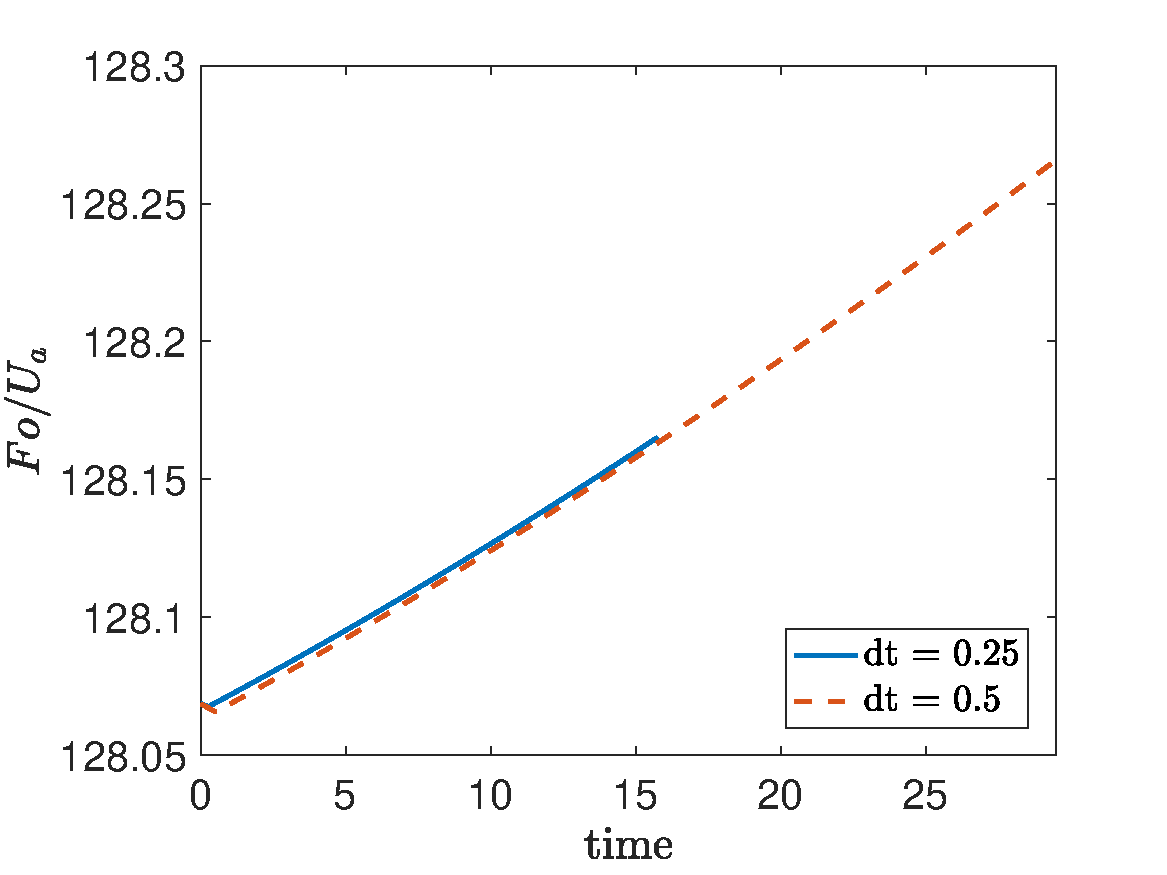
\includegraphics[scale=0.33]{./figures/fig_NC50_compare_dt_UaFo3_ratio}
		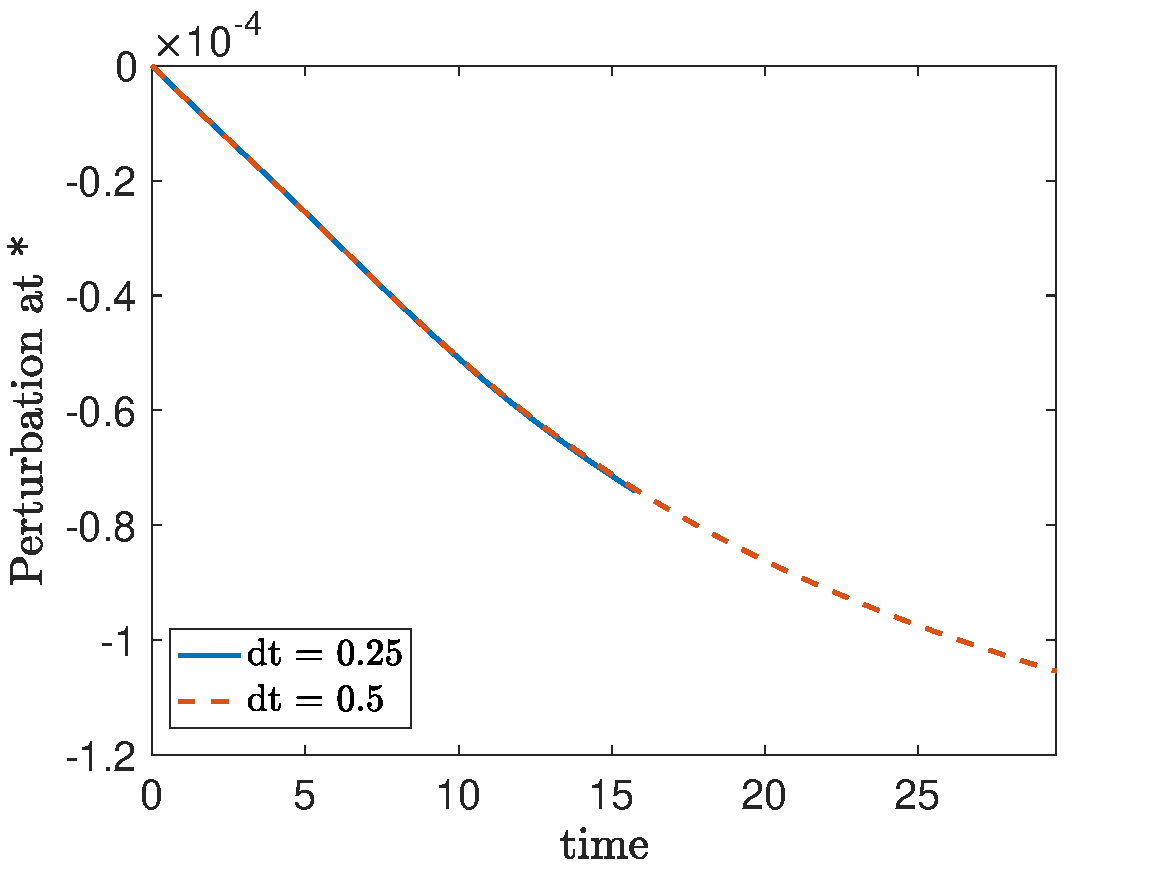
\includegraphics[scale=0.33]{./figures/fig_NC50_compare_dt_C_all}
	\caption{Compare two cases: }
	\label{fig_NC50_compare}
\end{center}
\end{figure}
\section{Discussions}